%%%%%%%%%%%%%%%%%%%%%%%%%%%%%%%%%%%%%%%%%
% Classicthesis Typographic Thesis
% LaTeX Template
% Version 1.4 (1/1/16)
%
% This template has been downloaded from:
% http://www.LaTeXTemplates.com
%
% Original author:
% André Miede (http://www.miede.de) with commenting modifications by:
% Vel (vel@LaTeXTemplates.com)
%
% License:
% GNU General Public License (v2)
%
% General Tips:
% 1) Make sure to edit the classicthesis-config.file
% 2) New enumeration (A., B., C., etc in small caps): \begin{aenumerate} \end{aenumerate}
% 3) For margin notes: \marginpar or \graffito{}
% 4) Do not use bold fonts in this style, it is designed around them
% 5) Use tables as in the examples
% 6) See classicthesis-preamble.sty for useful commands
%
%%%%%%%%%%%%%%%%%%%%%%%%%%%%%%%%%%%%%%%%%

%----------------------------------------------------------------------------------------
%	PACKAGES AND OTHER DOCUMENT CONFIGURATIONS
%----------------------------------------------------------------------------------------

\documentclass[
		twoside,openright,titlepage,numbers=noenddot,headinclude,%1headlines,
	 	footinclude=true,cleardoublepage=empty,
		dottedtoc, % Make page numbers in the table of contents flushed right with dots leading to them
		BCOR=2mm,paper=a4,fontsize=10pt, % Binding correction, paper type and font size
		ngerman,dutch, % Languages, change this to your language(s)
		]{scrreprt}

% Includes the file which contains all the document configurations and packages - make sure to edit this file
%%%%%%%%%%%%%%%%%%%%%%%%%%%%%%%%%%%%%%%%%
% Classicthesis Typographic Thesis
% Configuration File
%
% This file has been downloaded from:
% http://www.LaTeXTemplates.com
%
% Original author:
% André Miede (http://www.miede.de) with extensive commenting changes by:
% Vel (vel@LaTeXTemplates.com)
%
% License:
% GNU General Public License (v2)
%
% Important note:
% The main lines to change in this file are in the DOCUMENT VARIABLES
% section, the rest of the file is for advanced configuration.
%
%%%%%%%%%%%%%%%%%%%%%%%%%%%%%%%%%%%%%%%%%

%----------------------------------------------------------------------------------------
%	CHARACTER ENCODING
%----------------------------------------------------------------------------------------

\PassOptionsToPackage{utf8}{inputenc} % Set the encoding of your files. UTF-8 is the only sensible encoding nowadays. If you can't read äöüßáéçèê∂åëæƒÏ€ then change the encoding setting in your editor, not the line below. If your editor does not support utf8 use another editor!
\usepackage{inputenc}

%----------------------------------------------------------------------------------------
%	DOCUMENT VARIABLES
%	Fill in the lines below to enter your information into the thesis template
%	Each of the commands can be cited anywhere in the thesis
%----------------------------------------------------------------------------------------

% Remove drafting to get rid of the '[ Date - classicthesis version 4.0 ]' text at the bottom of every page
\PassOptionsToPackage{eulerchapternumbers,listings,drafting, pdfspacing, subfig,beramono,eulermath,parts}{classicthesis}
% Available options: drafting parts nochapters linedheaders eulerchapternumbers beramono eulermath pdfspacing minionprospacing tocaligned dottedtoc manychapters listings floatperchapter subfig

\newcommand{\myTitle}{A Classic Thesis Style\xspace}
\newcommand{\mySubtitle}{An Homage to The Elements of Typographic Style\xspace}
\newcommand{\myDegree}{Doktor-Ingenieur (Dr.-Ing.)\xspace}
\newcommand{\myName}{André Miede\xspace}
\newcommand{\myProf}{Put name here\xspace}
\newcommand{\myOtherProf}{Put name here\xspace}
\newcommand{\mySupervisor}{Put name here\xspace}
\newcommand{\myFaculty}{Put data here\xspace}
\newcommand{\myDepartment}{Put data here\xspace}
\newcommand{\myUni}{Put data here\xspace}
\newcommand{\myLocation}{Saarbrücken\xspace}
\newcommand{\myTime}{September 2015\xspace}
\newcommand{\myVersion}{version 4.2\xspace}

%----------------------------------------------------------------------------------------
%	USEFUL COMMANDS
%----------------------------------------------------------------------------------------

\newcommand{\ie}{i.\,e.}
\newcommand{\Ie}{I.\,e.}
\newcommand{\eg}{e.\,g.}
\newcommand{\Eg}{E.\,g.} 

\newcounter{dummy} % Necessary for correct hyperlinks (to index, bib, etc.)
\providecommand{\mLyX}{L\kern-.1667em\lower.25em\hbox{Y}\kern-.125emX\@}
\newlength{\abcd} % for ab..z string length calculation

%----------------------------------------------------------------------------------------
%	PACKAGES
%----------------------------------------------------------------------------------------

\usepackage{lipsum} % Used for inserting dummy 'Lorem ipsum' text into the template

%------------------------------------------------

%\PassOptionsToPackage{ngerman,american}{babel}  % Change this to your language(s)
% Spanish languages need extra options in order to work with this template
%\PassOptionsToPackage{spanish,es-lcroman}{babel}
\usepackage{babel}

%------------------------------------------------			

\usepackage{csquotes}
\PassOptionsToPackage{%
%backend=biber, % Instead of bibtex
backend=bibtex8,bibencoding=ascii,%
language=auto,%
style=numeric-comp,%
%style=authoryear-comp, % Author 1999, 2010
%bibstyle=authoryear,dashed=false, % dashed: substitute rep. author with ---
sorting=nyt, % name, year, title
maxbibnames=10, % default: 3, et al.
%backref=true,%
natbib=true % natbib compatibility mode (\citep and \citet still work)
}{biblatex}
\usepackage{biblatex}
 
 %------------------------------------------------

\PassOptionsToPackage{fleqn}{amsmath} % Math environments and more by the AMS 
 \usepackage{amsmath}
 
 %------------------------------------------------

\PassOptionsToPackage{T1}{fontenc} % T2A for cyrillics
\usepackage{fontenc}

%------------------------------------------------

\usepackage{textcomp} % Fix warning with missing font shapes

%------------------------------------------------

\usepackage{scrhack} % Fix warnings when using KOMA with listings package  

%------------------------------------------------

\usepackage{xspace} % To get the spacing after macros right

%------------------------------------------------

\usepackage{mparhack} % To get marginpar right

%------------------------------------------------

\usepackage{fixltx2e} % Fixes some LaTeX stuff 

%------------------------------------------------

\PassOptionsToPackage{smaller}{acronym} % Include printonlyused in the first bracket to only show acronyms used in the text
\usepackage{acronym} % Nice macros for handling all acronyms in the thesis

%\renewcommand*{\acsfont}[1]{\textssc{#1}} % For MinionPro
\renewcommand*{\aclabelfont}[1]{\acsfont{#1}}

%------------------------------------------------

\PassOptionsToPackage{pdftex}{graphicx}
\usepackage{graphicx} 

%----------------------------------------------------------------------------------------
%	FLOATS: TABLES, FIGURES AND CAPTIONS SETUP
%----------------------------------------------------------------------------------------

\usepackage{tabularx} % Better tables
\setlength{\extrarowheight}{3pt} % Increase table row height
\newcommand{\tableheadline}[1]{\multicolumn{1}{c}{\spacedlowsmallcaps{#1}}}
\newcommand{\myfloatalign}{\centering} % To be used with each float for alignment
\usepackage{caption}
\captionsetup{font=small}
\usepackage{subfig}  

%----------------------------------------------------------------------------------------
%	CODE LISTINGS SETUP
%----------------------------------------------------------------------------------------

\usepackage{listings} 
%\lstset{emph={trueIndex,root},emphstyle=\color{BlueViolet}}%\underbar} % For special keywords
\lstset{language=[LaTeX]Tex,%C++ % Specify the language(s) for listings here
morekeywords={PassOptionsToPackage,selectlanguage},
keywordstyle=\color{RoyalBlue}, % Add \bfseries for bold
basicstyle=\small\ttfamily, % Makes listings a smaller font size and a different font
%identifierstyle=\color{NavyBlue}, % Color of text inside brackets
commentstyle=\color{Green}\ttfamily, % Color of comments
stringstyle=\rmfamily, % Font type to use for strings
numbers=left, % Change left to none to remove line numbers
numberstyle=\scriptsize, % Font size of the line numbers
stepnumber=5, % Increment of line numbers
numbersep=8pt, % Distance of line numbers from code listing
showstringspaces=false, % Sets whether spaces in strings should appear underlined
breaklines=true, % Force the code to stay in the confines of the listing box
%frameround=ftff, % Uncomment for rounded frame
%frame=single, % Frame border - none/leftline/topline/bottomline/lines/single/shadowbox/L
belowcaptionskip=.75\baselineskip % Space after the "Listing #: Desciption" text and the listing box
}

%----------------------------------------------------------------------------------------
%	HYPERREFERENCES
%----------------------------------------------------------------------------------------

\PassOptionsToPackage{pdftex,hyperfootnotes=false,pdfpagelabels}{hyperref}
\usepackage{hyperref}  % backref linktocpage pagebackref
\pdfcompresslevel=9
\pdfadjustspacing=1

\hypersetup{
% Uncomment the line below to remove all links (to references, figures, tables, etc), useful for b/w printouts
%draft, 
colorlinks=true, linktocpage=true, pdfstartpage=3, pdfstartview=FitV,
% Uncomment the line below if you want to have black links (e.g. for printing black and white)
%colorlinks=false, linktocpage=false, pdfborder={0 0 0}, pdfstartpage=3, pdfstartview=FitV, 
breaklinks=true, pdfpagemode=UseNone, pageanchor=true, pdfpagemode=UseOutlines,%
plainpages=false, bookmarksnumbered, bookmarksopen=true, bookmarksopenlevel=1,%
hypertexnames=true, pdfhighlight=/O,%nesting=true,%frenchlinks,%
urlcolor=webbrown, linkcolor=RoyalBlue, citecolor=webgreen, %pagecolor=RoyalBlue,%
    %urlcolor=Black, linkcolor=Black, citecolor=Black, %pagecolor=Black,%
%------------------------------------------------
% PDF file meta-information
pdftitle={\myTitle},
pdfauthor={\textcopyright\ \myName, \myUni, \myFaculty},
pdfsubject={},
pdfkeywords={},
pdfcreator={pdfLaTeX},
pdfproducer={LaTeX with hyperref and classicthesis}
%------------------------------------------------
}

%----------------------------------------------------------------------------------------
%	AUTOREFERENCES SETUP
%	Redefines how references in text are prefaced for different 
%	languages (e.g. "Section 1.2" or "section 1.2")
%----------------------------------------------------------------------------------------

\makeatletter
\@ifpackageloaded{babel}
{
\addto\extrasamerican{
\renewcommand*{\figureautorefname}{Figure}
\renewcommand*{\tableautorefname}{Table}
\renewcommand*{\partautorefname}{Part}
\renewcommand*{\chapterautorefname}{Chapter}
\renewcommand*{\sectionautorefname}{Section}
\renewcommand*{\subsectionautorefname}{Section}
\renewcommand*{\subsubsectionautorefname}{Section}
}
\addto\extrasngerman{
\renewcommand*{\paragraphautorefname}{Absatz}
\renewcommand*{\subparagraphautorefname}{Unterabsatz}
\renewcommand*{\footnoteautorefname}{Fu\"snote}
\renewcommand*{\FancyVerbLineautorefname}{Zeile}
\renewcommand*{\theoremautorefname}{Theorem}
\renewcommand*{\appendixautorefname}{Anhang}
\renewcommand*{\equationautorefname}{Gleichung}
\renewcommand*{\itemautorefname}{Punkt}
}
\providecommand{\subfigureautorefname}{\figureautorefname} % Fix to getting autorefs for subfigures right
}{\relax}
\makeatother

%----------------------------------------------------------------------------------------

\usepackage{classicthesis} 

%----------------------------------------------------------------------------------------
%	CHANGING TEXT AREA 
%----------------------------------------------------------------------------------------

%\linespread{1.05} % a bit more for Palatino
%\areaset[current]{312pt}{761pt} % 686 (factor 2.2) + 33 head + 42 head \the\footskip
%\setlength{\marginparwidth}{7em}%
%\setlength{\marginparsep}{2em}%

%----------------------------------------------------------------------------------------
%	USING DIFFERENT FONTS
%----------------------------------------------------------------------------------------

%\usepackage[oldstylenums]{kpfonts} % oldstyle notextcomp
%\usepackage[osf]{libertine}
%\usepackage[light,condensed,math]{iwona}
%\renewcommand{\sfdefault}{iwona}
%\usepackage{lmodern} % <-- no osf support :-(
%\usepackage{cfr-lm} % 
%\usepackage[urw-garamond]{mathdesign} <-- no osf support :-(
%\usepackage[default,osfigures]{opensans} % scale=0.95 
%\usepackage[sfdefault]{FiraSans}

\addbibresource{Bibliography.bib} % The file housing your bibliography
%\addbibresource[label=ownpubs]{Self_Publications.bib} % Uncomment for optional self-publications

%\hyphenation{Put special hyphenation here}


\begin{document}

\frenchspacing % Reduces space after periods to make text more compact

\raggedbottom % Makes all pages the height of the text on that page

\selectlanguage{dutch} % Select your default language - e.g. american or ngerman

%\renewcommand*{\bibname}{new name} % Uncomment to change the name of the bibliography
%\setbibpreamble{} % Uncomment to include a preamble to the bibliography - some text before the reference list starts

\pagenumbering{roman} % Roman page numbering prior to the start of the thesis content (i, ii, iii, etc)

\pagestyle{plain} % Suppress headers for the pre-content pages

%----------------------------------------------------------------------------------------
%	PRE-CONTENT THESIS PAGES
%----------------------------------------------------------------------------------------

% Title Page

\begin{titlepage}

\begin{addmargin}[-1cm]{-3cm}
\begin{center}
\large

\hfill
\vfill

\begingroup
\color[HTML]{27406B}\spacedallcaps{\myTitle} \\ \bigskip % Thesis title

\color[HTML]{84C6C8}\mySubtitle \\ \medskip
\endgroup

\spacedlowsmallcaps{\myName} % Your name

\vfill


\includegraphics[width=15cm]{gfx/EagleScience_Logo_on_white} \\  % Picture

 % Thesis subtitle
%\myDegree \\

\myworkName \\
\myworkAddress \\
\myworkPostcodeCity \\ \bigskip \bigskip \bigskip

\myTime\ -- \myVersion % Time and version

\vfill

\end{center}
\end{addmargin}

\end{titlepage}
 % Main title page

% Back of the title page

\thispagestyle{empty}

\hfill

\vfill

\noindent\myName: \textit{\myTitle,} \mySubtitle, %\myDegree, 
\textcopyright\ \myTime

% You may wish to do something with the back of the title page, such as including your supervisors, location or time frame of the work. Below is an example of doing so although you may want to tweak it to your liking.

%\bigskip

%\noindent\spacedlowsmallcaps{Supervisors}: \\
%\myProf \\
%\myOtherProf \\ 
%\mySupervisor

%\medskip \\

%\noindent\spacedlowsmallcaps{Location}: \\
%\myLocation

%\medskip \\

%\noindent\spacedlowsmallcaps{Time Frame}: \\
%\myTime
 % Back of the title page

%\cleardoublepage% Dedication

\thispagestyle{empty}
\refstepcounter{dummy}

\pdfbookmark[1]{Dedication}{Dedication} % Bookmark name visible in a PDF viewer

\vspace*{3cm}

\begin{center}
\emph{Ohana} means family. \\
Family means nobody gets left behind, or forgotten. \\ \medskip
--- Lilo \& Stitch    
\end{center}

\medskip

\begin{center}
Dedicated to the loving memory of Rudolf Miede. \\ \smallskip
1939\,--\,2005
\end{center} % Dedication page

%\cleardoublepage\include{FrontBackMatter/Foreword} % Uncomment and create a Foreword.tex to include a foreword

\cleardoublepage% Abstract

%\renewcommand{\abstractname}{Abstract} % Uncomment to change the name of the abstract

\pdfbookmark[1]{Abstract}{Abstract} % Bookmark name visible in a PDF viewer

\begingroup
\let\clearpage\relax
\let\cleardoublepage\relax
\let\cleardoublepage\relax

\chapter*{Samenvating}
Eaglescience is een bedrijf dat innovatieve software maakt wat poogt de wereld te verbeteren. Het bedrijf is opzoek naar een methode om periodiek een automatische SOUP analyse te doen op zowel bestaande projecten als projecten die nog in ontwikkeling is. Er wordt in dit onderzoek gezocht naar die methode waarbij gekeken wordt naar een mogelijke off-the-shelf oplossing en bij het niet vinden hiervan een oplossing die in-house wordt ontwikkelt door ondergetekende. \\
Om inzicht te krijgen in SOUP en een analyse hierop wordt er eerst een onderzoek gedaan naar de verschillende begrippen binnen het domijn SOUP zodat er een beter beeld ontstaat in de wensen van Eaglescience. 

\endgroup			

\vfill % Abstract page

%\cleardoublepage% Publications - a page listing research articles written using content in the thesis

\pdfbookmark[1]{Publications}{Publications} % Bookmark name visible in a PDF viewer

\chapter*{Publications} % Publications page text

Some ideas and figures have appeared previously in the following publications:\\

\noindent Put your publications from the thesis here. The packages \texttt{multibib} or \texttt{bibtopic} etc. can be used to handle multiple different bibliographies in your document.

%\begin{refsection}[ownpubs]
%    \small
%    \nocite{*} % is local to to the enclosing refsection
%    \printbibliography[heading=none]
%\end{refsection}

%\emph{Attention}: This requires a separate run of \texttt{bibtex} for your \texttt{refsection}, \eg, \texttt{ClassicThesis1-blx} for this file. You might also use \texttt{biber} as the backend for \texttt{biblatex}. See also \url{http://tex.stackexchange.com/questions/128196/problem-with-refsection}. % Publications from the thesis page

%\cleardoublepage% Acknowledgements

\pdfbookmark[1]{Acknowledgements}{Acknowledgements} % Bookmark name visible in a PDF viewer

\begin{flushright}{\slshape    
We have seen that computer programming is an art, \\ 
because it applies accumulated knowledge to the world, \\ 
because it requires skill and ingenuity, and especially \\
because it produces objects of beauty.} \\ \medskip
--- \defcitealias{knuth:1974}{Donald E. Knuth}\citetalias{knuth:1974} \citep{knuth:1974}
\end{flushright}

\bigskip

%----------------------------------------------------------------------------------------

\begingroup

\let\clearpage\relax
\let\cleardoublepage\relax
\let\cleardoublepage\relax

\chapter*{Acknowledgements}

\noindent Put your acknowledgements here.\\

\noindent Many thanks to everybody who already sent me a postcard!\\

\noindent Regarding the typography and other help, many thanks go to Marco Kuhlmann, Philipp Lehman, Lothar Schlesier, Jim Young, Lorenzo Pantieri and Enrico Gregorio\footnote{Members of GuIT (Gruppo Italiano Utilizzatori di \TeX\ e \LaTeX )}, J\"org Sommer, Joachim K\"ostler, Daniel Gottschlag, Denis Aydin, Paride Legovini, Steffen Prochnow, Nicolas Repp, Hinrich Harms, Roland Winkler, and the whole \LaTeX-community for support, ideas and some great software.

\bigskip

\noindent\emph{Regarding \mLyX}: The \mLyX\ port was initially done by
\emph{Nicholas Mariette} in March 2009 and continued by
\emph{Ivo Pletikosi\'c} in 2011. Thank you very much for your work and the contributions to the original style.

\endgroup % Acknowledgements page

\pagestyle{scrheadings} % Show chapter titles as headings

\cleardoublepage% Table of Contents - List of Tables/Figures/Listings and Acronyms

\refstepcounter{dummy}

\pdfbookmark[1]{\contentsname}{tableofcontents} % Bookmark name visible in a PDF viewer

\setcounter{tocdepth}{2} % Depth of sections to include in the table of contents - currently up to subsections

\setcounter{secnumdepth}{3} % Depth of sections to number in the text itself - currently up to subsubsections

\manualmark
\markboth{\spacedlowsmallcaps{\contentsname}}{\spacedlowsmallcaps{\contentsname}}
\tableofcontents 
\automark[section]{chapter}
\renewcommand{\chaptermark}[1]{\markboth{\spacedlowsmallcaps{#1}}{\spacedlowsmallcaps{#1}}}
\renewcommand{\sectionmark}[1]{\markright{\thesection\enspace\spacedlowsmallcaps{#1}}}

\clearpage

\begingroup 
\let\clearpage\relax
\let\cleardoublepage\relax
\let\cleardoublepage\relax

%----------------------------------------------------------------------------------------
%	List of Figures
%----------------------------------------------------------------------------------------

\refstepcounter{dummy}
%\addcontentsline{toc}{chapter}{\listfigurename} % Uncomment if you would like the list of figures to appear in the table of contents
\pdfbookmark[1]{\listfigurename}{lof} % Bookmark name visible in a PDF viewer

\listoffigures

\vspace{8ex}
\newpage

%----------------------------------------------------------------------------------------
%	List of Tables
%----------------------------------------------------------------------------------------

\refstepcounter{dummy}
%\addcontentsline{toc}{chapter}{\listtablename} % Uncomment if you would like the list of tables to appear in the table of contents
\pdfbookmark[1]{\listtablename}{lot} % Bookmark name visible in a PDF viewer

\listoftables
        
\vspace{8ex}
\newpage
    
%----------------------------------------------------------------------------------------
%	List of Listings
%---------------------------------------------------------------------------------------- 

\refstepcounter{dummy}
%\addcontentsline{toc}{chapter}{\lstlistlistingname} % Uncomment if you would like the list of listings to appear in the table of contents
\pdfbookmark[1]{\lstlistlistingname}{lol} % Bookmark name visible in a PDF viewer

\lstlistoflistings 

\vspace{8ex}
\newpage
       
%----------------------------------------------------------------------------------------
%	Acronyms
%----------------------------------------------------------------------------------------

\refstepcounter{dummy}
%\addcontentsline{toc}{chapter}{Acronyms} % Uncomment if you would like the acronyms to appear in the table of contents
\pdfbookmark[1]{Acronyms}{acronyms} % Bookmark name visible in a PDF viewer

\markboth{\spacedlowsmallcaps{Acronyms}}{\spacedlowsmallcaps{Acronyms}}

\chapter*{Acronyms}

\begin{acronym}[UML]
\acro{DRY}{Don't Repeat Yourself}
\acro{API}{Application Programming Interface}
\acro{UML}{Unified Modeling Language}
\end{acronym}  
                   
\endgroup % Contents, list of figures/tables/listings and acronyms

\cleardoublepage

\pagenumbering{arabic} % Arabic page numbering for thesis content (1, 2, 3, etc)
%\setcounter{page}{90} % Uncomment to manually start the page counter at an arbitrary value (for example if you wish to count the pre-content pages in the page count)

\cleardoublepage % Avoids problems with pdfbookmark

%----------------------------------------------------------------------------------------
%	THESIS CONTENT - CHAPTERS
%----------------------------------------------------------------------------------------

% Text on the Part 1 page describing  the content in Part 1

% Chapter X

\chapter{Inleiding}\label{ch:inleiding} % Chapter title
\textbf{Als laatste schrijven}

\lipsum[01-03]
 % inleiding

\ctparttext{}
\part{Idee}\label{prt:idee} % First part of the thesis
% Chapter 1
\chapter{Eaglescience}\label{ch:eaglescience} % Chapter title

\label{ch:Eaglescience} % For referencing the chapter elsewhere, use \autoref{ch:introduction}

%----------------------------------------------------------------------------------------

Het hier beschreven onderzoek en de daarbij behorende applicatie is geschreven in opdracht van het bedrijf Eaglescience wat gevestigd is in Amsterdam Sloterdijk.
Eaglescience ontwikkeld complexe software op projectbasis voor diverse klanten.
Deze projecten hebben meestal een wetenschappelijke inslag.
Hiernaast biedt Eaglescience ook de mogelijkheid aan de klant om zorg te dragen voor de eventuele hosting van het opgeleverde product.
Eaglescience kan hierdoor nog beter garanderen dat de geboden kwaliteit in de software gewaarborgd blijft tijdens de levensduur van de software.

\section{Organisatie}\label{sec:organisatie}
\marginpar{Organisatie}

Eaglescience BV bestaat uit drie divisies: Innovations, Software en Solutions [figuurX].%besxchrijving van de drie takken
Het bestaat op het moment van schrijven uit $\pm$ 20 medewerkers waarvan 75\% verantwoordelijk is voor de ontwikkeling van de geleverde software.
De andere 25\% bekleed een support rol zoals project manager, finance manager, quality manager, automatisering etc. \\

\begin{figure}[bth]
\myfloatalign
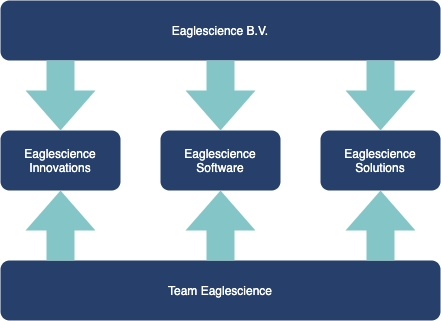
\includegraphics[width=10cm]{gfx/organogram}
\caption{Organogram Eaglescience}
\label{fig:Eaglescience organogram}
\end{figure}
% vragen Wat zijn de hoofddoelen van iedere divisie?
% betere verwoording vragen:
De divisie Eaglescience Innovations zoekt naar nieuwe oplossingen op het gebied van softwareontwikkeling, deze worden door de divisie Eaglescience software geïmplementeerd.
Eaglescience Solutions is een divisie die samen met de klant op zoek gaat naar een oplossing voor een gesteld probleem.\\
Het dagelijks bestuur is handen van:
\begin{itemize}
\item CEO / CFO - Marc Grootjen
\item CTO - Bas Breier
\item COO - Wender van Mansvelt \\
\end{itemize}
Onder het dagelijks bestuur valt Team Eaglescience wat bestaat uit projectmanagers en ontwikkelaars.
Deze zijn onderverdeeld in diverse scrum teams die ieders verantwoordelijk zijn voor een project.
De ontwikkelaars worden parallel ingezet op meerdere projecten om kennisdeling te bevorderen.

\section{missie}\label{sec:missie}
\marginpar{Missie}
De missie van Eaglescience is het bedienen van haar partners door een ontwerp, ontwikkeling en service te bieden op het gebied van op maat gemaakte IT-oplossingen.
Om hier voor te zorgen heeft Eaglescience goed opgeleide IT-professionals in dienst die zichzelf continue ontwikkelen op de “cutting edge” van IT-technologie.
De hoofd competenties van de medewerkers zijn: innovatief, intelligent, klant georiënteerd, flexibel en ambitieus.

\section{visie}\label{sec:visie}
Eaglescience streeft er als innovatief IT bedrijf naar om software te ontwikkelen als een Business-to-Business dienst.
Middels technische vaardigheden bouwen we veilige en hoogwaardige software die bijdraagt aan een betere wereld.
Omdat we agile werken, leveren we precies wat nodig is, niets meer en niets minder.
Wij helpen onze klanten zoeken naar een langdurige betrokkenheid en samenwerking op basis van zowel vertrouwen als wederzijds respect. \\
\marginpar{Visie}
Omdat elke vraag uniek is, ontwikkeld Eaglescience op maar gemaakte en innovatieve software.
We zijn van plan deel uit te maken van het hele proces van het formuleren van een idee tot het lanceren van het product en het waarborgen van de productie levenscyclus.
Onze belangrijkste succesfactor zijn de mensen, die zich continu ontwikkelen door met de nieuwste technieken te werken op diverse projecten.
Wij streven naar een optimale balans tussen werk en privé.
Dit geeft onze medewerkers veel vrijheid, maar vereist zelfdiscipline en verantwoordelijkheid.

\section{strategie}\label{sec:strategie}
Eaglescience levert de visie via vier strategische thema's:
\begin{itemize}
    \item Maatschappelijke verantwoordelijkheid
    \item Persoonlijke groei
    \item Tevredenheid
    \item 4e???? %Wender vragen
\end{itemize}
\marginpar{strategische thema's}
We streven ernaar om veilige en hoogwaardige software diensten te leveren die waarde toevoegen aan onze samenleving.
We streven naar een bedrijfscultuur waarin alle collega's hun talenten kunnen laten groeien.
We hebben een ongecompliceerd werkethos: we richten ons op resultaten van hoge kwaliteit, maar met een gezonde balans tussen werk en privé en voldoende tijd voor leuke en sociale evenementen.
Eaglescience verwacht van alle medewerkers dat zij hun handelen baseren op vier kwaliteitsprincipes:
\begin{itemize}
    \item Meld situaties die niet voldoen aan onze interne procedures
    \item Evalueer risico's wanneer grote veranderingen worden verwacht
    \item Help en daag elkaar uit
    \item Kennis behouden over compliancy en kwaliteitsmanagement
\end{itemize}

\section{Werkwijze}\label{sec:werkwijze}
Zoals eerder gemeld werkt Eaglescience op projectbasis met ontwikkelaars in meerdere teams.
Er wordt geprobeerd "Full scrum" te werken waarbij de requirements van de klant centraal staan.
Als een project wordt aangenomen door het managementteam dan wordt deze in sprints in samenspraak met de klant ontwikkeld.
De klant wordt nauw betrokken bij het verloop van de ontwikkeling door het geven van demo's aan het einde van iedere sprint.
Hier wordt gemeten hoe de applicatie zich gedraagt met betrekking tot de requirements van de klant.
Dit is ook het moment dat er feedback gegeven wordt en waar nodig gestuurd kan worden in het verdere verloop.
Op het moment dat er een applicatie klaar is wordt de software al dan niet overgedragen aan de klant of doorgegeven aan support en hosting die verantwoordelijk zijn voor de daadwerkelijke hosting van de software.
\begin{figure}[bth]
\myfloatalign
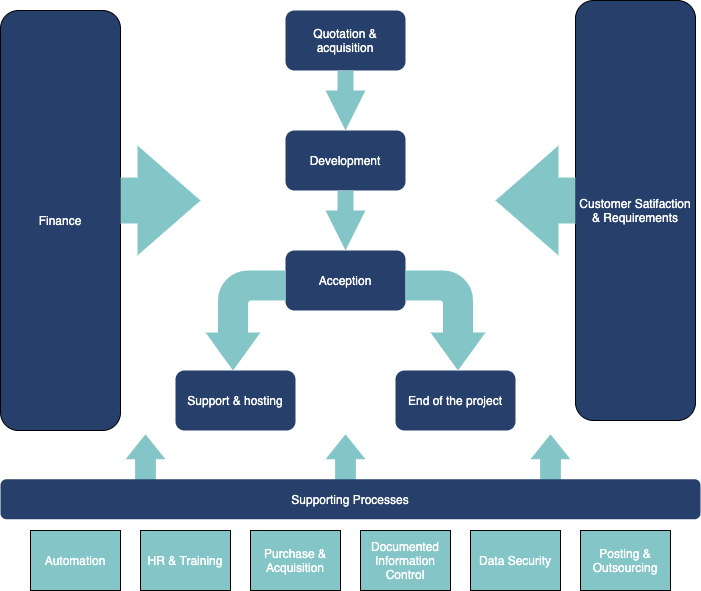
\includegraphics[width=10cm]{gfx/ProcessFlow}
\caption{Project Process}
\label{fig:Project Process}
\end{figure}

Naast het ontwikkel process zijn er een aantal supporting processen die ervoor zorgdragen dat het bedrijf blijft draaien en er nieuwe mensen aangenomen kunnen worden.
Maar ook een deel automatisering die voor ondersteuning zorgt van platformen waarop ontwikkeld en of gehosted wordt.\\
Eaglescience ontwikkeld op projectbasis en op die manier worden er ook inkomsten gegenereerd.
Alle processen die draaien moeten dus ingezet kunnen worden op projecten van klanten.
Als er een project voor in huis gebruik wordt ondernomen moet er een duidelijk beeld zijn of er op termijn winst mee te behalen is op monetair vlak dan al niet tijdswinst of ontwikkel gemak.

\section{Relevante en actuele ontwikkelingen binnen Eaglescience}\label{sec:relevante-en-actuele-ontwikkelingen-binnen-eaglescience}
Eaglescience is aan het groeien, zowel in het aantal projecten waar aan gewerkt wordt als het aantal medewerkers.
Daarnaast worden de diensten die Eaglescience aanbied ook uitgebreid, en wordt het hosten van de ontwikkelde applicaties steeds vaker aangeboden.
Door deze inzet ligt de verantwoordelijkheid niet alleen bij het leveren van een veilige en hoogwaardige software, maar ook bij het leveren van een veilige hosting service.
Mede door de groei van het bedrijf maar zeker ook de diensten die aangeboden wordt is het belangrijk om taken die geautomatiseerd kunnen dan ook te automatiseren.
 % Chapter 1 Eaglescience
% Chapter 1

\chapter{Idee}\label{ch:idee}

Wachtrijen zijn het meest irritante tijdverdrijf bij het bezoek van aan een pret  /themepark tijd dus om dit aan te pakken. en volgen ons zijn er twee manieren om dit te doen:


Een mogelijk is ook het gebruik van een "Fast Pass" systeem waarbij gasten middels een reservatie systeem tijdslots kunnen reservere


\section{wachtrijen fysiek aanpassen}\label{sec:wachtrijen-fysiek-aanpassen}


\section{Wachtrijen virtueel maken}\label{sec:wachtrijen-virtueel-maken}
De voordelen van het maken van virtuele wachtrijen geeft de bezoeker een
zodat je in iedergeval een soort van vrijheid ervaart}
Wat als je nooit langer dan 10 minuten in een wachtrij hoeft te wachten in een pretpark. De wachtrijen die men nu


This template for \LaTeX\ has two goals:
\begin{enumerate}
\item Provide students with an easy-to-use template for their Master's or PhD thesis (though it might also be used by other types of authors for reports, books, etc.).
\item Provide a classic, high-quality typographic style that is inspired by \citeauthor{bringhurst:2002}'s ``\emph{The Elements of Typographic Style}'' \citep{bringhurst:2002}.
\marginpar{\myTitle \myVersion}
\end{enumerate}

The bundle is configured to run with a \emph{full} MiK\TeX\ or \TeX Live installation right away and, therefore, it uses only freely available fonts.

People interested only in the nice style and not the whole bundle can now use the style stand-alone via the file \texttt{classicthesis.sty}. This works now also with ``plain'' \LaTeX.

As of version 3.0, \texttt{classicthesis} can also be easily used with \mLyX\footnote{\url{http://www.lyx.org}} thanks to Nicholas Mariette and Ivo Pletikosi\'c. The \mLyX\ version of this manual will contain more information on the details.

This should enable anyone with a basic knowledge of \LaTeXe\ or \mLyX\ to produce beautiful documents without too much effort. In the end, this is my overall goal: more beautiful documents, especially theses, as I am tired of seeing so many ugly ones.

The whole template and the used style is released under the \textsmaller{GNU} General Public License. 

If you like the style then I would appreciate a postcard:
\begin{center}
André Miede \\
Detmolder Straße 32 \\
31737 Rinteln \\
Germany
\end{center}

\noindent The postcards I received so far are available at:
\begin{center}
 \url{http://postcards.miede.de}
\end{center}
\marginpar{A well-balanced line width improves the legibility of the text. That's what typography is all about, right?} So far, many theses, some books, and several other publications have been typeset successfully with it. If you are interested in some typographic details behind it, enjoy Robert Bringhurst's wonderful book. % \citep{bringhurst:2002}.

\paragraph{Important Note:} Some things of this style might look unusual at first glance, many people feel so in the beginning. However, all things are intentionally designed to be as they are, especially these:
\begin{itemize}
\item No bold fonts are used. Italics or spaced small caps do the job quite well.
\item The size of the text body is intentionally shaped like it is. It supports both legibility and allows a reasonable amount of information to be on a page. And, no: the lines are not too short.
\item The tables intentionally do not use vertical or double rules. See the documentation for the \texttt{booktabs} package for a nice discussion of this topic.\footnote{To be found online at \\ \url{http://www.ctan.org/tex-archive/macros/latex/contrib/booktabs/}.}
\item And last but not least, to provide the reader with a way easier access to page numbers in the table of contents, the page numbers are right behind the titles. Yes, they are \emph{not} neatly aligned at the right side and they are \emph{not} connected with dots that help the eye to bridge a distance that is not necessary. If you are still not convinced: is your reader interested in the page number or does she want to sum the numbers up?
\end{itemize}

\noindent Therefore, please do not break the beauty of the style by changing these things unless you really know what you are doing! Please.

\paragraph{Yet Another Important Note:} Since \texttt{classicthesis}' first release in 2006, many things have changed in the \LaTeX\ world.  Trying to keep up-to-date, \texttt{classicthesis} grew and evolved into many directions, trying to stay (some kind of) stable and be compatible with its port to \mLyX. However, there are still many remains from older times in the code, many dirty workarounds here and there, and several other things I am absolutely not proud of (for example my unwise combination of \acsfont{KOMA} and \texttt{titlesec} etc.). \graffito{An outlook into the future of \texttt{classicthesis}.}

Currently, I am looking into how to completely re-design and re-implement \texttt{classicthesis} making it easier to maintain and to use. As a general idea, \texttt{classicthesis.sty} should be developed and distributed separately from the template bundle itself. Excellent spin-offs such as \texttt{arsclassica} could also be integrated (with permission by their authors) as format configurations. Also, current trends of \texttt{microtype}, \texttt{fontspec}, etc. should be included as well. As I am not really into deep \LaTeX\ programming, I will reach out to the \LaTeX\ community for their expertise and help.

%----------------------------------------------------------------------------------------

\section{Organization}
A very important factor for successful thesis writing is the organization of the material. This template suggests a structure as the following:
\begin{itemize}
\marginpar{You can use these margins for summaries of the text body\dots}
\item\texttt{Chapters/} is where all the ``real'' content goes in separate files such as \texttt{Chapter01.tex} etc.
\item\texttt{FrontBackMatter/} is where all the stuff goes that surrounds the ``real'' content, such as the acknowledgments, dedication, etc.
\item\texttt{gfx/} is where you put all the graphics you use in the thesis. Maybe they should be organized into subfolders depending on the chapter they are used in, if you have a lot of graphics.
\item\texttt{Bibliography.bib}: the Bib\TeX\ database to organize all the references you might want to cite.
\item\texttt{classicthesis.sty}: the style definition to get this awesome look and feel. Bonus: works with both \LaTeX\ and \textsc{pdf}\LaTeX\dots and \mLyX.
\item\texttt{ClassicThesis.tcp} a \TeX nicCenter project file. Great tool and it's free!
\item\texttt{ClassicThesis.tex}: the main file of your thesis where all the content gets bundled together.
\item\texttt{classicthesis-config.tex}: a central place to load all nifty packages that are used. In there, you can also activate backrefs in order to have information in the bibliography about where a source was cited in the text (\ie, the page number).
    
\emph{Make your changes and adjustments here.} This means that you specify here the options you want to load \texttt{classicthesis.sty} with. You also adjust the title of your thesis, your name, and all similar information here. Refer to \autoref{sec:custom} for more information.

This had to change as of version 3.0 in order to enable an easy transition from the ``basic'' style to \mLyX.
\end{itemize}

\noindent In total, this should get you started in no time.

%----------------------------------------------------------------------------------------

\section{Style Options}\label{sec:options}

There are a couple of options for \texttt{classicthesis.sty} that allow for a bit of freedom concerning the layout: \marginpar{\dots or your supervisor might use the margins for some comments of her own while reading.}
\begin{itemize}
\item General:
\begin{itemize}
\item\texttt{drafting}: prints the date and time at the bottom of each page, so you always know which version you are dealing with. Might come in handy not to give your Prof. that old draft.
\end{itemize}
	
\item Parts and Chapters:
\begin{itemize}
\item\texttt{parts}: if you use Part divisions for your document, you should choose this option. (Cannot be used together with \texttt{nochapters}.)

\item\texttt{nochapters}: allows to use the look-and-feel with classes that do not use chapters, \eg, for articles. Automatically turns off a couple of other options: \texttt{eulerchapternumbers}, \texttt{linedheaders}, \texttt{listsseparated}, and \texttt{parts}. 

\item\texttt{linedheaders}: changes the look of the chapter headings a bit by adding a horizontal line above the chapter title. The chapter number will also be moved to the top of the page, above the chapter title.
\end{itemize}

\item Typography:
\begin{itemize}
\item\texttt{eulerchapternumbers}: use figures from Hermann Zapf's Euler math font for the chapter numbers. By default, old style figures from the Palatino font are used.

\item\texttt{beramono}: loads Bera Mono as typewriter font. (Default setting is using the standard CM typewriter font.)

\item\texttt{eulermath}: loads the awesome Euler fonts for math. (Palatino is used as default font.)

\item\texttt{pdfspacing}: makes use of pdftex' letter spacing capabilities via the \texttt{microtype} package.\footnote{Use \texttt{microtype}'s \texttt{DVIoutput} option to generate DVI with pdftex.} This fixes some serious issues regarding math formul\ae\ etc. (\eg, ``\ss'') in headers. 

\item\texttt{minionprospacing}: uses the internal \texttt{textssc} command of the \texttt{MinionPro} package for letter spacing. This automatically enables the \texttt{minionpro} option and overrides the \texttt{pdfspacing} option.
\end{itemize}  

\item Table of Contents:
\begin{itemize}
\item\texttt{tocaligned}: aligns the whole table of contents on the left side. Some people like that, some don't.

\item\texttt{dottedtoc}: sets pagenumbers flushed right in the table of contents.

\item\texttt{manychapters}: if you need more than nine chapters for your document, you might not be happy with the spacing between the chapter number and the chapter title in the Table of Contents. This option allows for additional space in this context. However, it does not look as ``perfect'' if you use \verb|\parts| for structuring your document.
\end{itemize}

\item Floats:
\begin{itemize}
\item\texttt{listings}: loads the \texttt{listings} package (if not already done) and configures the List of Listings accordingly.
    
\item\texttt{floatperchapter}: activates numbering per chapter for all floats such as figures, tables, and listings (if used).	
    
\item\texttt{subfig}(\texttt{ure}): is passed to the \texttt{tocloft} package to enable compatibility with the \texttt{subfig}(\texttt{ure}) package. Use this option if you want use classicthesis with the \texttt{subfig} package.

\end{itemize}    

\end{itemize}

\noindent The best way to figure these options out is to try the different possibilities and see, what you and your supervisor like best.

In order to make things easier in general, \texttt{classicthesis-config.tex} contains some useful commands that might help you.

%----------------------------------------------------------------------------------------

\section{Customization}\label{sec:custom}

This section will give you some hints about how to adapt \texttt{classicthesis} to your needs.

The file \texttt{classicthesis.sty} contains the core functionality of the style and in most cases will be left intact, whereas the file \texttt{classic\-thesis-config.tex} is used for some common user customizations. 

The first customization you are about to make is to alter the document title, author name, and other thesis details. In order to do this, replace the data in the following lines of \texttt{classicthesis-config.tex:}\marginpar{Modifications in \texttt{classic\-thesis-config.tex}
}

\begin{lstlisting}
\newcommand{\myTitle}{A Classic Thesis Style\xspace}
\newcommand{\mySubtitle}{An Homage to ...\xspace}
\end{lstlisting}

Further customization can be made in \texttt{classicthesis-config.tex} by choosing the options to \texttt{classicthesis.sty} (see~\autoref{sec:options}) in a line that looks like this:

\begin{lstlisting}
\PassOptionsToPackage{eulerchapternumbers,listings,drafting, pdfspacing, subfig,beramono,eulermath,parts}{classicthesis}
\end{lstlisting}

Many other customizations in \texttt{classicthesis-config.tex} are possible, but you should be careful making changes there, since some changes could cause errors.

Finally, changes can be made in the file \texttt{classicthesis.sty}, \marginpar{Modifications in \texttt{classicthesis.sty}} although this is mostly not designed for user customization. The main change that might be made here is the text-block size, for example, to get longer lines of text.

%----------------------------------------------------------------------------------------

\section{Issues}\label{sec:issues}
This section will list some information about problems using \texttt{classic\-thesis} in general or using it with other packages.

Beta versions of \texttt{classicthesis} can be found at Bitbucket:
\begin{center}
    \url{https://bitbucket.org/amiede/classicthesis/}
\end{center}
There, you can also post serious bugs and problems you encounter.

\subsection*{Compatibility with the \texttt{glossaries} Package}
If you want to use the \texttt{glossaries} package, take care of loading it with the following options:
\begin{verbatim}
\usepackage[style=long,nolist]{glossaries}
\end{verbatim}

\noindent Thanks to Sven Staehs for this information. 

\subsection*{Compatibility with the (Spanish) \texttt{babel} Package}
Spanish languages need an extra option in order to work with this template:
\begin{lstlisting}
    \usepackage[spanish,es-lcroman]{babel}
\end{lstlisting}
Thanks to an unknown person for this information (via the issue reporting). 

\paragraph{Further information for using \texttt{classicthesis} with Spanish (in addition to the above)}
In the file \texttt{ClassicThesis.tex} activate the language: 
\begin{lstlisting}
    \selectlanguage{spanish}
\end{lstlisting}

If there are issues changing \verb|\tablename|, \eg, using this:
\begin{lstlisting}
    \renewcommand{\tablename}{Tabla}
\end{lstlisting}

This can be solved by passing \texttt{es-tabla} parameter to \texttt{babel}:
\begin{lstlisting}
    \PassOptionsToPackage{es-tabla,spanish,es-lcroman,english}{babel}
    \usepackage{babel}
\end{lstlisting}

But it is also necessary to set \texttt{spanish} in the \verb|\documentclass|.

Thanks to Alvaro Jaramillo Duque for this information. 

\subsection*{Compatibility with the \texttt{pdfsync} Package}
Using the \texttt{pdfsync} package leads to linebreaking problems with the \texttt{graffito} command. Thanks to Henrik Schumacher for this information. 

%----------------------------------------------------------------------------------------

\section{Future Work}
So far, this is a quite stable version that served a couple of people well during their thesis time. However, some things are still not as they should be. Proper documentation in the standard format is still missing. In the long run, the style should probably be published separately, with the template bundle being only an application of the style. Alas, there is no time for that at the moment\dots it could be a nice task for a small group of \LaTeX nicians.

Please do not send me email with questions concerning \LaTeX\ or the template, as I do not have time for an answer. But if you have comments, suggestions, or improvements for the style or the template in general, do not hesitate to write them on that postcard of yours.

%----------------------------------------------------------------------------------------

\section{Beyond a Thesis}
The layout of \texttt{classicthesis.sty} can be easily used without the framework of this template. A few examples where it was used to typeset an article, a book or a curriculum vitae can be found in the folder \texttt{Examples}. The examples have been tested with \texttt{latex} and \texttt{pdflatex} and are easy to compile. To encourage you even more, PDFs built from the sources can be found in the same folder.

%----------------------------------------------------------------------------------------

\section{License}
\paragraph{GNU General Public License:} This program is free software; you can redistribute it and/or modify it under the terms of the \textsmaller{GNU} General Public License as published by the Free Software Foundation; either version 2 of the License, or (at your option) any later version.

This program is distributed in the hope that it will be useful, but \emph{without any warranty}; without even the implied warranty of \emph{merchantability} or \emph{fitness for a particular purpose}. See the \textsmaller{GNU} General Public License for more details.
 % Chapter 2 Opdracht
% Chapter 1
\chapter{Eaglescience}\label{ch:eaglescience} % Chapter title

\label{ch:Eaglescience} % For referencing the chapter elsewhere, use \autoref{ch:introduction}

%----------------------------------------------------------------------------------------

Het hier beschreven onderzoek en de daarbij behorende applicatie is geschreven in opdracht van het bedrijf Eaglescience wat gevestigd is in Amsterdam Sloterdijk.
Eaglescience ontwikkeld complexe software op projectbasis voor diverse klanten.
Deze projecten hebben meestal een wetenschappelijke inslag.
Hiernaast biedt Eaglescience ook de mogelijkheid aan de klant om zorg te dragen voor de eventuele hosting van het opgeleverde product.
Eaglescience kan hierdoor nog beter garanderen dat de geboden kwaliteit in de software gewaarborgd blijft tijdens de levensduur van de software.

\section{Organisatie}\label{sec:organisatie}
\marginpar{Organisatie}

Eaglescience BV bestaat uit drie divisies: Innovations, Software en Solutions [figuurX].%besxchrijving van de drie takken
Het bestaat op het moment van schrijven uit $\pm$ 20 medewerkers waarvan 75\% verantwoordelijk is voor de ontwikkeling van de geleverde software.
De andere 25\% bekleed een support rol zoals project manager, finance manager, quality manager, automatisering etc. \\

\begin{figure}[bth]
\myfloatalign
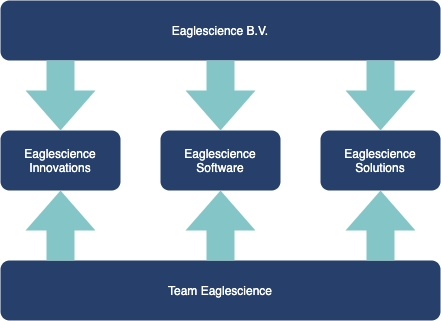
\includegraphics[width=10cm]{gfx/organogram}
\caption{Organogram Eaglescience}
\label{fig:Eaglescience organogram}
\end{figure}
% vragen Wat zijn de hoofddoelen van iedere divisie?
% betere verwoording vragen:
De divisie Eaglescience Innovations zoekt naar nieuwe oplossingen op het gebied van softwareontwikkeling, deze worden door de divisie Eaglescience software geïmplementeerd.
Eaglescience Solutions is een divisie die samen met de klant op zoek gaat naar een oplossing voor een gesteld probleem.\\
Het dagelijks bestuur is handen van:
\begin{itemize}
\item CEO / CFO - Marc Grootjen
\item CTO - Bas Breier
\item COO - Wender van Mansvelt \\
\end{itemize}
Onder het dagelijks bestuur valt Team Eaglescience wat bestaat uit projectmanagers en ontwikkelaars.
Deze zijn onderverdeeld in diverse scrum teams die ieders verantwoordelijk zijn voor een project.
De ontwikkelaars worden parallel ingezet op meerdere projecten om kennisdeling te bevorderen.

\section{missie}\label{sec:missie}
\marginpar{Missie}
De missie van Eaglescience is het bedienen van haar partners door een ontwerp, ontwikkeling en service te bieden op het gebied van op maat gemaakte IT-oplossingen.
Om hier voor te zorgen heeft Eaglescience goed opgeleide IT-professionals in dienst die zichzelf continue ontwikkelen op de “cutting edge” van IT-technologie.
De hoofd competenties van de medewerkers zijn: innovatief, intelligent, klant georiënteerd, flexibel en ambitieus.

\section{visie}\label{sec:visie}
Eaglescience streeft er als innovatief IT bedrijf naar om software te ontwikkelen als een Business-to-Business dienst.
Middels technische vaardigheden bouwen we veilige en hoogwaardige software die bijdraagt aan een betere wereld.
Omdat we agile werken, leveren we precies wat nodig is, niets meer en niets minder.
Wij helpen onze klanten zoeken naar een langdurige betrokkenheid en samenwerking op basis van zowel vertrouwen als wederzijds respect. \\
\marginpar{Visie}
Omdat elke vraag uniek is, ontwikkeld Eaglescience op maar gemaakte en innovatieve software.
We zijn van plan deel uit te maken van het hele proces van het formuleren van een idee tot het lanceren van het product en het waarborgen van de productie levenscyclus.
Onze belangrijkste succesfactor zijn de mensen, die zich continu ontwikkelen door met de nieuwste technieken te werken op diverse projecten.
Wij streven naar een optimale balans tussen werk en privé.
Dit geeft onze medewerkers veel vrijheid, maar vereist zelfdiscipline en verantwoordelijkheid.

\section{strategie}\label{sec:strategie}
Eaglescience levert de visie via vier strategische thema's:
\begin{itemize}
    \item Maatschappelijke verantwoordelijkheid
    \item Persoonlijke groei
    \item Tevredenheid
    \item 4e???? %Wender vragen
\end{itemize}
\marginpar{strategische thema's}
We streven ernaar om veilige en hoogwaardige software diensten te leveren die waarde toevoegen aan onze samenleving.
We streven naar een bedrijfscultuur waarin alle collega's hun talenten kunnen laten groeien.
We hebben een ongecompliceerd werkethos: we richten ons op resultaten van hoge kwaliteit, maar met een gezonde balans tussen werk en privé en voldoende tijd voor leuke en sociale evenementen.
Eaglescience verwacht van alle medewerkers dat zij hun handelen baseren op vier kwaliteitsprincipes:
\begin{itemize}
    \item Meld situaties die niet voldoen aan onze interne procedures
    \item Evalueer risico's wanneer grote veranderingen worden verwacht
    \item Help en daag elkaar uit
    \item Kennis behouden over compliancy en kwaliteitsmanagement
\end{itemize}

\section{Werkwijze}\label{sec:werkwijze}
Zoals eerder gemeld werkt Eaglescience op projectbasis met ontwikkelaars in meerdere teams.
Er wordt geprobeerd "Full scrum" te werken waarbij de requirements van de klant centraal staan.
Als een project wordt aangenomen door het managementteam dan wordt deze in sprints in samenspraak met de klant ontwikkeld.
De klant wordt nauw betrokken bij het verloop van de ontwikkeling door het geven van demo's aan het einde van iedere sprint.
Hier wordt gemeten hoe de applicatie zich gedraagt met betrekking tot de requirements van de klant.
Dit is ook het moment dat er feedback gegeven wordt en waar nodig gestuurd kan worden in het verdere verloop.
Op het moment dat er een applicatie klaar is wordt de software al dan niet overgedragen aan de klant of doorgegeven aan support en hosting die verantwoordelijk zijn voor de daadwerkelijke hosting van de software.
\begin{figure}[bth]
\myfloatalign
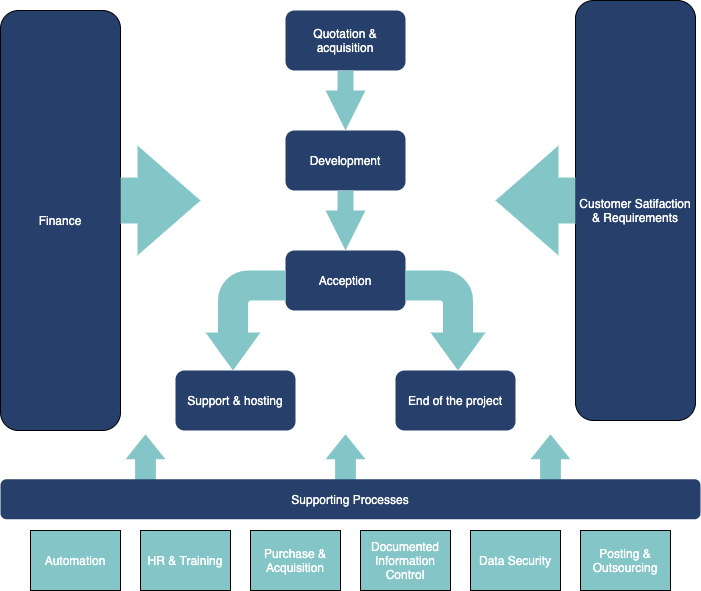
\includegraphics[width=10cm]{gfx/ProcessFlow}
\caption{Project Process}
\label{fig:Project Process}
\end{figure}

Naast het ontwikkel process zijn er een aantal supporting processen die ervoor zorgdragen dat het bedrijf blijft draaien en er nieuwe mensen aangenomen kunnen worden.
Maar ook een deel automatisering die voor ondersteuning zorgt van platformen waarop ontwikkeld en of gehosted wordt.\\
Eaglescience ontwikkeld op projectbasis en op die manier worden er ook inkomsten gegenereerd.
Alle processen die draaien moeten dus ingezet kunnen worden op projecten van klanten.
Als er een project voor in huis gebruik wordt ondernomen moet er een duidelijk beeld zijn of er op termijn winst mee te behalen is op monetair vlak dan al niet tijdswinst of ontwikkel gemak.

\section{Relevante en actuele ontwikkelingen binnen Eaglescience}\label{sec:relevante-en-actuele-ontwikkelingen-binnen-eaglescience}
Eaglescience is aan het groeien, zowel in het aantal projecten waar aan gewerkt wordt als het aantal medewerkers.
Daarnaast worden de diensten die Eaglescience aanbied ook uitgebreid, en wordt het hosten van de ontwikkelde applicaties steeds vaker aangeboden.
Door deze inzet ligt de verantwoordelijkheid niet alleen bij het leveren van een veilige en hoogwaardige software, maar ook bij het leveren van een veilige hosting service.
Mede door de groei van het bedrijf maar zeker ook de diensten die aangeboden wordt is het belangrijk om taken die geautomatiseerd kunnen dan ook te automatiseren.


\ctparttext{}
\part{Onderzoek}\label{prt:Onderzoek} % Second part of the thesis
% Chapter 3

\chapter{Inleiding}\label{ch:inleiding3} % Chapter title

\label{inOnderzoek} % For referencing the chapter elsewhere, use \autoref{ch:InOnderzoek}
Op basis van de requirements analyse beschreven in het vorige deel zijn er een aantal vragen ontstaan die verder onderzoek benodigd behoeven.
In dit deel worden de vragen geanalyseerd en beantwoord zodat er een duidelijkheid is in de materie en een goede basis wordt gelegd voor de daadwerkelijke implementatie beschreven in het volgende deel.

\section{Scope}\label{sec:scope}
Het onderzoek zal zich beperken tot de benodigde informatie voor het implementeren van de nieuwe oplossing voor een geautomatiseerde SOUP analyse.
Het zal ingaan op de gebruikte ontwikkelstack binnen Eaglescience en bestaande architectuur gezien de nieuwe oplossing een onderdeel is van een al bestaand project en hier dus naadloos op moet integreren.
Daarnaast zal er onderzoek gedaan worden naar wat een SOUP-analyse daadwerkelijk is en welke problemen het mogelijk op kan lossen.
Met daarbij een mogelijke oplossingen om een SOUP analyse te kunnen doen.

Gezien de vragen in twee verschillende domeinen gesteld worden is het ook noodzakelijk om deze vragen op te delen in twee onderzoeken.
In de komende hoofdstukken zal er dan ook voor ieder domein een eigen onderzoek worden beschreven met daarin de resultaten die vervolgens gebruikt kunnen worden voor de implementatie die volgt in een volgend deel.

De volgende onderwerpen worden in deze hoofdstukken beschreven:
\begin{itemize}
    \item Onderzoeksmethode, een beschrijving van de gebruikte methoden en aanpak van de beide onderzoeken.
    \item Onderzoek: Architectuur binnen eaglescience, een onderzoek naar de gebruikte architectuur binnen Eaglescience alsook de werkwijze waarop Eaglescience software ontwikkeld.
    \item Onderzoek: SOUP-analyse, een onderzoek over wat SOUP precies is welke gevaren er potentieel mee gemoeid gaan, en welke oplossingen er bestaan om SOUP-analyses te doen.
\end{itemize}

% Chapter 3

\chapter{Onderzoeksmethode}\label{ch:onderzoeksmethode} % Chapter title

Zoals in de inleiding vermeld zijn er twee onderzoeken benodigd om deze opdracht te kunnen volbrengen.
In de komende secties is te vinden welke methode, stategiën en scoping zijn gebruikt om een resultaat te vinden.
Waarbij iedere sectie een onderzoek vertegenwoordigd


\section{Onderzoek: Architectuur binnen Eaglescience}\label{sec:onderzoeksmethode-architectuur-binnen-eaglescience}
Het resultaat van dit onderzoek moet zijn: "Het hebben van inzicht in de manier van werken binnen Eaglescience en de daarbij horende keuzes voor ontwikkeltalen, architectuur, en tools".
Om deze inzicht te krijgen is het volgende onderzoeksmodel (figuur:\ref{fig:Onderzoeks model Eaglescience}) opgesteld waarbij er vanuit eigen kennis, interne workshops en vooronderzoek gekeken is naar gebruikte ontwikkelingstalen en tooling.
Deze is vervolgens geverifieerd met senior developers.
Hieruit is vervolgens het resultaat in de vorm van inzicht in de huidige dev-stack naar voren gekomen.
\begin{figure}[h!] %todo: Nog in kleur zetten van Eaglescience als deze goed is.
  \myfloatalign
  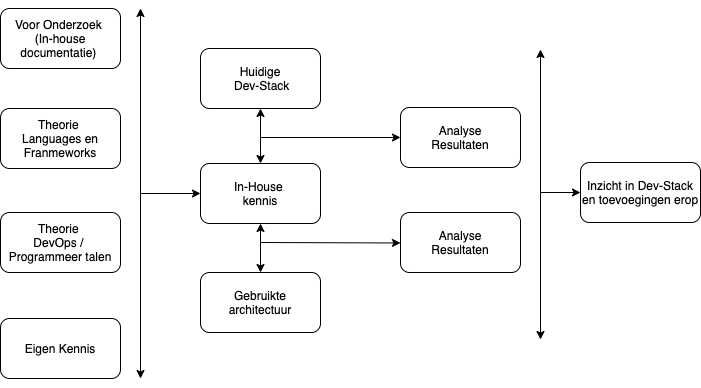
\includegraphics[width=10cm]{gfx/OnderzoeksmodelES}
  \caption{Onderzoeksmodel Eaglescience}
  \label{fig:Onderzoeks model Eaglescience}
\end{figure}

Zoals vermeld is er eerst vanuit eigen kennis, vooronderzoek en kennis opgedaan in de door Eaglescience workshops een lijst gemaakt met de gebruikte technieken.
Daarna is deze geverifieerd met senior ontwikkelaars doormiddel van interviews.
Tijdens deze interviews is ook ruimte geweest voor de reden en filosofie achter de keuzes die er gemaakt zijn in het gebruik van de talen.

\section{Onderzoek naar SOUP-analyse}\label{sec:onderzoek-naar-soup-analyse}
Dit onderzoek heeft als ingang het gegeven dat er kwetsbaarheden in de bibliotheken zitten met daarbij de dev-stack van Eaglescience.
Het resultaat van dit onderzoek moet zijn dat er een methode moet zijn waarbij er een assesment op de bestaande dev-stack binnen de werkwijze van Eaglescience moet komen die geimplementeerd kan worden.
Het onderzoekmodel (figuur:\ref{fig:Onderzoeks model Dev-Stack}) geeft weer dat de ingangs kennis de opgedane kennis uit het onderzoek naar de architectuur van Eaglescience en een literatuur studie naar mogelijkheden om soup te analyseren.

\begin{figure}[h!] %Todo: Nog in kleur zetten van Eaglescience als deze goed is.
  \myfloatalign
  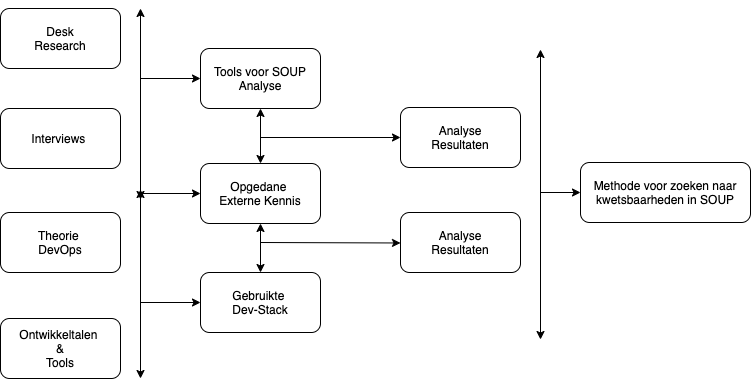
\includegraphics[width=10cm]{gfx/OnderzoeksmodelSOUP}
  \caption{Onderzoeksmodel SOUP analyse module}
  \label{fig:Onderzoeks model Dev-Stack}
\end{figure}

Veel kennis van buiten zal worden vergaard doormiddel van het lezen van artikelen en boeken over het onderwerp.
Hierbij moet worden gelet op de toepasbaarheid en scope van het artikel.

\section{Tijdsverloop Onderzoeken}\label{sec:tijdsverloop-onderzoeken}
Beide onderzoeken zullen parallel uitgevoerd worden zodat beide onderzoeken elkaar inzichten kunnen verschaffen en er op die manier een beter begrip van de mogelijkheden is.

%! Author = bas
%! Date = 24/08/2021

% Preamble
\documentclass[11pt]{article}

% Packages
\usepackage{amsmath}

% Document
\begin{document}



\end{document}

% Chapter X

\chapter{Onderzoek: SOUP analyse}\label{ch:onderzoek:-soup-analyse} % Chapter title

\begin{itemize}
\item https://jeremylong.github.io/DependencyCheck/
\end{itemize}

Voordat we verder kijken naar mogelijkheden om kwetsbaarheden in een externe bibliotheek te onderzoeken en te verhelpen moeten we eerst kijken naar een aantal kernbegrippen om te begrijpen waar het om gaat.

Dit onderzoek heeft daarom ook twee hoofdvragen die ieders weer een aantal deelvragen opwerpen.
Als eeste is de vraag "Welke kwetsbaarheden bestaan er hoe is het gebruik van externe bibliotheken hier aan gecorreleerd?
De deelvragen die hier uit voorkomen luiden:
\begin{itemize}
  \item Wat zijn applicatie veiligheidsrisico's?
  \item Welke komen het meest voor?
  \item
\end{itemize}

\section{Wat zijn applicatie veiligheidsrisico's}\label{sec:wat-zijn-applicatie-veiligheids-risico's}
Veiligheids risico's binnen applicaties zijn een som van kwetsbaarheden die zich bedoeld of onbedoeld in de applicatie bevinden, de vindbaarheid en de "schade" die er mee aangericht kunnen worden.
De termen van de som worden hieronder verder uitgediept als ook een top-10 uitgeven door de OWASP van de meest voorkomende kwetbaarheden.

Een aanvaller kan op meerdere manier in een applicatie komen(figuur X).
Vaak gebeurt dit door een kwetsbaarheid van een applicatie te zoeken en deze te exploiteren.
Als er vervolgens geen maatregeling genomen zijn om de aanvaller te weerhouden kunnen er zaken als data in een database, assets van het bedrijf of zelfs functionaliteit aangetast worden.
Wat op zijn beurt weer voor een impact in de bedrijfsvoering kan veroorzaken.
Hoe aanvallers een applicatie kunnen aanvallen is applicatie specifiek
De impact op de bedrijfsvoering is ook specifiek
\begin{figure}[H]
  \myfloatalign
  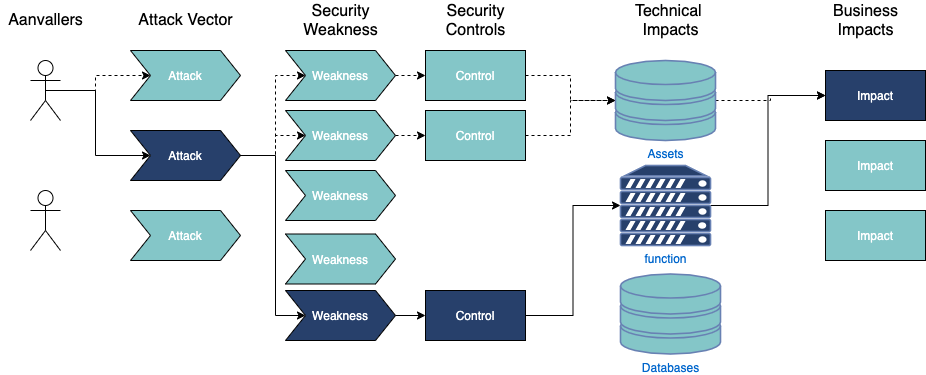
\includegraphics[width=15cm]{gfx/application security routes}
  \caption{Aanvalllen, en hun gevolg}
  \label{fig:Application Security Routes}
\end{figure}

Veiligheids risico's kunnen in categoriën worden geplaatst middels een gradatie systeem die in figuur x te ze zien is.
De OWASP-Top10 die verder in de tekst te vinden is maakt gebruik van dit gradatie systeem om risico's in te schalen.
OWASP is een instantie die zich bezighouden met het verbeteren van de veiligheid van applicaties.
Het doet dit door onder andere training en erkenning te geven aan kwetsbaarheden.
Zo wordt er eens in de 5 jaar een top-10 samengesteld met de op dat moment meest voorkomende kwetsbaarheden.
\footnote{Helaas is de laatste versie die aan het einde van 2021 uit moet komen nog niet beschikbaar op het moment van schrijven}
De OWASP-Top10 wordt samengesteld uit data van meer dan 100.000 productie applicaties en APIs wat door meer dan 500 mensen is getest door 40 verschillende bedrijven.
De top 10 is een aggegratie van deze data in de meest voorkomende issues met inachtneming van exploitabity, detectability en impact.


\begin{figure}[H]
  \myfloatalign
  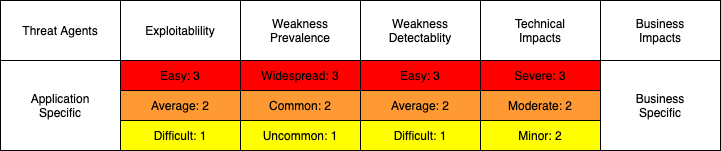
\includegraphics[width=12cm]{gfx/risk tabel}
  \caption{Inschaling van risico's}
  \label{fig:risico inschaling}
\end{figure}

%threat agents = aanvallende entiteit
%exploitabity = exploiteetbaatheid
%weakness prevalance = vookomendheid van de zwakte in een applicatie
%weakness detectability = hoe goed is de zwakte in een applicatie te detecteren
%technical impact = technische impact op de applicaties
%business impacts = (zakelijke impact) impact op de bedrijfsvoering

\begin{itemize}

%Bron: https://codebros.nl/blog/wat-is-de-owasp-top-10 , https://owasp.org/www-project-top-ten/ << PDF download

  \item \textbf{A01:2017 Injection [exploitabity: 3, Prevelance: 2, detectability: 3, technical: 3] :} \\
  De mogelijkheid om OS, SQL, NoSQL commandos te injecteren in web applicaties zorgt ervoor dat aanvallers toegang kunnen hebben tot delen van systemen zonder er recht op te hebben.\ Daarnaast is er ook de mogelijkheid om toegang te krijgen tot data die niet voor hen bedoelt is.

  \item \textbf{A02:2017 Broken Authentication [exploitabity: 3, Prevelance: 2, detectability: 2, technical: 3]:}\\ Het verkeerd implementeren van authentication en session management kan er voor zorgen dat aanvallers wachtwoorden, sessie tokens aan kunnen passen om zo zich voor te doen als een andere gebruiker.

  \item \textbf{A03:2017 Sensitive Data Exposure [exploitabity: 2, Prevelance: 3, detectability: 2, technical: 3]:}\\
  Het verkeerd of niet voldoende afschermen van APIs kunnen ervoor zorgen dat sensitive data makkelijk gevonden kan worden.\ Zeker als de data niet encrypted verzonden wordt.

  \item \textbf{A04:2017 XML External Entities (XXE) [exploitabity: 2, Prevelance: 2, detectability: 3, technical: 3]:}\\
  Veel oude of slecht geconfigureerde XML-processoren evalueren externe entiteit referenties binnen XML documenten slecht. Hierdoor is het mogelijk om links te cree\"en naar bestanden en/of fileshares waar code staat die slecht is voor de applicatie [that contains malicious code].

  \item \textbf{A05:2017 Broken Access Control [exploitabity: 2, Prevelance: 2, detectability: 2, technical: 3]:}\\
  Restricties op wat een geauthenticeerde gebruikers mogen worden niet altijd nageleefd, Aanvallers kunnend deze fouten gebruiken om toegang te krijgen tot gegevens of functionaliteiten die niet bestemd zijn voor deze gebruikers. Ze kunnen gegevens aanpassen en of toegangsrechten aanpassen.

  \item \textbf{A06:2017 Security Misconfiguration [exploitabity: 3, Prevelance: 3, detectability: 3, technical: 2]:}\\
  Slechte configuratie van de veiligheids instellingen zijn de meest gevonden ??issue??. Dit is meestal het gevolg van het gebruiken van de default, incomplete of ad-hoc configuratie Hierdoor kunnen cloud storages open komen te staan, verkeerd geconfigureerde HTTP headers of foutmeldingen die te veel informatie meegeven ontstaan.

  \item \textbf{A07:2017 Cross-Site Scripting (XSS) [exploitabity: 3, Prevelance: 3, detectability: 3, technical: 2]:}\\ middels XSS is het mogelijk om scripts te draaien van een andere bron dan wenselijk. Dit geeft de mogelijkheid om via een browser andere scripts in de applicatie te draaien zo proberen andere functionaliteiten toe te voegen. Wat kan resulteren in een web site dat zich anders gedraagt dan de bedoeling is.

  \item \textbf{A08:2017 Insecure Deserialization [exploitabity: 1, Prevelance: 2, detectability: 2, technical: 3]:}\\ Door het niet veilig serialiseren van objecten naar text kan het voorkomen dat er code of commando's mee worden gestuurd welke uitgevoers kunnen worden op de server.

  \item \textbf{A09:2017 Using components with Known vulnerabilities [exploitabity: 2, Prevelance: 3, detectability: 2, technical: 2]:}\\
  Componenten zoals bibliotheken, frameworks en andere software modules die gebruikt worden voor het ontwikkelen van een applicatie kunnen bedoelt en of onbedoeld [malicious code ] bevatten Wat kan resulteren in verschillende mogelijkheden voor de aanvaller binnen te dringen. of data te versturen naar een andere host om zo achter "beveiligde" gegevens te komen.

  \item \textbf{A10:2017 Insuffivient Logging \& Monitoring[exploitabity: 2, Prevelance: 3, detectability: 1, technical: 2]:}\\
  Logging en monitoring is bijna net zo belangrijk als het ontwikkelen van een veilige applicatie, mocht er toch een aanval plaatsvinden op welke manier dient er de mogelijkheid zijn om terug te zien wat er precies gebeurt is. Logging zorgt hiervoor. Het monitoring deel is het bekijken van de logs om te zien of er iets verdachts plaats heeft gevonden. Er zijn tools beschikbaar die er voor automatische monitoring zorgen( Nagios is dit soort tool)

\end{itemize}


In het vorige hoofdstuk is te lezen dat Eaglescience gebruik maakt van de volgende technologi\"en: Scala 2.XX, TypeScript, Jenkins, Docker ,Azure cloud.

Dit onderzoek richt voornamelijk op kwetbaarheden in bibliotheken  van derden en de bestrijding ervan.
En specifiek op de bovenstaande door Eaglescience gebruikte technieken.
De hoofdvraag voor dit hoofdstuk luid dan ook: "Met welke kwetsbaarheden hebben we te maken binnen Eaglescience en hoe kunnen we deze opsporen op een automatiseerde manier zonder de huidige werkwijze te verstoren?" Uit deze hoofdvraag onstaan de volgende deelvragen die in dit onderzoek beantwoord worden met daarna een conclusie op de hoofdvraag.

\begin{itemize}
\item Welke soorten kwetsbaarheden zijn er?
\item Hoe kunnen deze kwetbaarheden hun weg vinden in onze gebouwde software?
\item Zijn er instanties die bijhouden waar zich kwetsbaarheden schuilhouden?
\item Wat zijn methodes om te onderzoeken of er in de bestaande software kwetbaarheden bevinden?
\item Is er een mogelijkheid om een third-party pakket in te zetten om dit te doen?
\end{itemize}

\

Binnen Eaglescience wordt er heel goed gekeken naar de manier waarop er veilige software ontwikkeld wordt.
Zaken die in de OWASP top-10 staan wordt serieus mee omgegaan en actief tegen gehandeld. zo wordt er ook gegekeken naar het gebruik van bibliotheken van derden.

Op plaats A09:2017 is te vinden dat er kwetsbaarheden middels bibliotheken van derden binnen kunnen komen. Dit is iets wat deels buiten het bereik van Eaglescience ligt. Om ons hier tegen te beschermen is het wenselijk om periodiek en geautomatiseerd een analyse naar kwetbaarheden tedoen.

De bibliotheken die gebruikt worden van derden wordt ook wel Software of unkown pedigree genoemd of kortweg SOUP. Dit houdt in dat een bibliotheek wordt ontwikkeld middels een proces of methode wat niet bekend is bij de eindgebruiker. Ook zijn vaak de details niet bekend van de bibliotheek omdat deze niet of nauwelijks wordt gereviewed door de eindgebruiker. Om deze reden is het dus onbekend of er kwetsbaarheden zitten in betreffende bibliotheken.
De definitie van SOUP blijft niet alleen bij de bibliotheken en frameworks vanuit het open-source gebied. Veelal is ook niet bekend hoe closed-source (Proprietary software) wordt geschreven, echter door reputatie van bedrijven die deze software schrijven wordt veelal , onterecht\footnote{zie: https://www.nu.nl/tech/6097701/waarom-de-hack-bij-solarwinds-ministeries-en-grote-bedrijven-treft.html } aangenomen dat deze geen lekken bevatten.

\section{CVE}
in de appliction security wordt er gesproken van een CVE(Common Vulnerability en Exposures) als een kewtsbaarheid bekend is deze wordt in een database geplaatst zodat \'e\'en ieder die geintreseerd is hier kan vinden welke software(os, applicatie, framework, bibliotheek) mogelijk niet veilig is. Deze Database wordt in stand en bijgehouden door een aantal instanties waarbij de belangrijksten zijn:
\begin{itemize}
  \item \textbf{NIST-CSRC} Computer Security Research Center van het National Institute of Standards and Technology) is een centrum dat onderzoek doet namens de Amerikaanse regering naar veiligheden in software. De database die het NIST-CSRC bijhoud heet het NVD(National Vulnerability Database) waarin CVE's worden bijgehouden.
  \item \textbf{CVE-Mitre} is een community driven effort wat CVE's logt in een lijst die vervolgens de NVD voedt met hun gevondendata.
  \item \textbf{cvedetails.com/}
  \item \textbf{vuldb.com/}
  \item \textbf{https://www.exploit-db.com/}
\end{itemize}

\section{}

https://www.security.nl/posting/666663/Van+CVE+tot+CVSS\%3A+wegwijs+in+het+woud+van+kwetsbaarheden










\section{Zijn er instanties die bijhouden waar zich kwetsbaarheden schuilhouden?}

Naast OWASP zijn er nog een aantal instanties dit bijhouden welke software\footnote{zoals hier gebruikt in de bereedste? zin van het woord dus: (Operating systems, ontwikkeltalen/databases, ontwikkelframeworks,bibliotheken) }
mogelijk kwetsbaarheden kunnen bevatten.
\begin{itemize}

\end{itemize}


\section{Wat zijn methodes om te onderzoeken of er in de bestaande software kwetbaarheden bevinden?}

\section{Is er een mogelijkheid om een third-party pakket in te zetten om dit te doen?}

% Chapter 2

\chapter{Conclusie} % Chapter title

\label{ch:onderzoekConclusie} % For referencing the chapter elsewhere, use \autoref{ch:examples}

Dit hoofdstuk zal de conclussies van beide onderzoeken samen zetten om samen tot een eind conclussie te komen waarop de ontwikkeling van de module kan worden gebasseerd.

\section{Conclusie Intern onderzoek Eaglescience}
Eaglescience werkt op project basis aan software voor de klant. Dit wordt gedaan op basis van "full scrum" waarbij er na iedere sprint een poging wordt gedaan om een (deels) werkende applicatie op te leveren. De applicaties die gebouwd worden zijn voornamelijk geschreven in Scala en TypeScript. De keuze voor Scala is voornamelijk gebaseerd op de mogelijkheid om condense, betrouwbare, voorspelbare en makkelijk te testen software te ontwikkelen. TypeScipt wat een superset set is van JavaScipt is gekozen omdat het de mogelijkheid bied om getypeert te programeren wat de foutgevoeligheid niet in de runtime legt maar al op het moment dat de code geschreven wordt.

Jenkins als build automator is een veelzijdige tool die het mogelijk maakt om een build process aan te passen aan de wensen van Eaglescience. Het is dus mogelijk om naast het gebruik van clair voor het scannen op kwetsbaarheden ook een andere stap toe te voegen die kijkt naar kwetsbaarheden binnen de ontwikkelde software.

\section{Conclusie SOUP analyses en theorie inbouwen van de module}
lekker
\lipsum[01]

\section{Conclusie van de onderzoeken genomen} %Wellicht in een enkele conclussie maken.

% Chapter X

\chapter{Onderzoek: Architectuur binnen Eaglescience}\label{ch:onderzoek:-architectuur-binnen-eaglescience} % Chapter title
 % For referencing the chapter elsewhere, use \autoref{ch:voorOnderzoek}
Dit onderzoek is een onderzoek binnen Eaglescience naar gebruikte technologiën welke dev-stack er gebruikt wordt.
Daarnaast wordt er gekeken naar de huidige manier van werken.
Het resultaat van dit onderzoek moet zijn dat er een beeld is over hoe er nu gewerkt wordt met welke technologiën.
Daarnaast moet er een beeld komen van de nieuwe situatie en hoe de nieuwe module in deze bestaande werkwijze past zonder veel aanpassingen.

Ook zal er worden onderzocht welke build pipeline er gebruikt wordty en of mogelijkheden zijn om deze aan te passen om een SOUP-analyse uit te kunnen voeren.an SOUP-Bibliotheken mogelijk kan maken.
\section{Onderzoeksvraag}\label{sec:onderzoeksvraag}
De onderzoeksvraag luid: "Hoe levert Eaglescience software, en wat moet er aangepast worden om de huidige manier om te zetten naar een manier waarbij er autmatisch een SOUP-analyse gedaan wordt?" Uit deze onderzoeksvraag komen een aantal deelvragen die verder in dit onderzoek zullen worden beantwoord.
Met als laatst het antwoord op de hoofvraag als resultaat.

\begin{itemize}
  \item Welk process wordt er gebruikt binnen Eaglescience om software te leveren aan de klant?
  \item Welke tooling en Ontwikkeltalen worden er gebruikt binnen eagleScience?
  \item Hoe wordt op dit moment de ontwikkelde software gedeployed?
  \item Welke architectuur wordt er op dit moment gebruikt in de portal?
  \item Waar wordt de software uiteindelijk gedeployed?
  \item Welke methoden zijn er buiten Eaglescience om te zien of een bibliotheek kwetsbaarheden bevat?
  \item Wat is Software of Unkown Pedigree?
\end{itemize}

\section{Interviews Teamleden Eaglescience}\label{sec:interviews-teamleden-eaglescience}
Om antwoorden te krijgen op de vragen die hierboven zijn uitgewerkt, zijn er interviews gehouden met een aantal personen binnen eaglescience.
De gesprekken zijn uitgewerkt in de secties hieronder.
De verslagen van de interviews zijn te vinden in Appendix A

\section{Hoe wordt er op het moment gewerkt binnen eagleScience?}\label{sec:hoe-wordt-er-op-het-moment-gewerkt-binnen-eaglescience?}
Eaglescience werkt op project basis met klanten, wat wil zeggen dat er in principe altijd een einde is gedefineerd.
Door dit gegeven kan er worden gewerkt in fasen die hieronder worden beschreven.
Er is een uitzondering op de laatste fase project maintenance.
Welke doorloopt tot de end-of-life van de software, of tot de klant de samenwerking stopzet.

\textbf{Phase1: Sales \& acquisition}
onderzoeksfase waarin vooral de wensen en restricutes vanuit de klant in kaart wordt gebracht.
Hierbij kan gedacht worden aan: Doel van de applicatie met daarbij de requirements en restraints, planning, budget en hosting.
Het resultaat is een inschattingsdocument met daarin informatie die het team verder helpt in het vormgeven van het project.

\textbf{Phase2: Project initiation}
In deze fase wordt het project opgestart.
Er wordt een team samengesteld die gaat werken aan het ontwikkelen van de software.
Deze fase is ook cruciaal om alle platform in gereedheid te brengen te denken aan rechten voor de ontwikkelaars op Azure Cloud, Sentri, Jenkins en dergelijke.
Als alles in gereedheid wordt gebracht is er een project kick-off waarbij hetteam wordt ingelicht over het project en taken die vervult moeten gaan worden.

\textbf{Phase3: Start \& Execution}
Dit is een iteratieve fase die in sprints doorloopt tot het project gereed is.
Waarbij na iedere sprint een demo wordt gegeven verdere uitweiding over deze fase is hieronder te vinden onder "Dagelijkse werkwijze"

\textbf{Phase4: Project Warp up}
In deze fase wordt het project opgeleverd aan de klant en wordt dan al niet door Eaglescience gehost op Azure cloud.
Er wordt een project retro gehouden waarbij het team terugkijkt op de werkzaamheden en hoe deze verliepen, daarnaast is er een evaluatie met de klant.

\textbf{Phase5: Project maintenance}
Geen enkel software wordt direct zonder bugs opgeleverd deze fase duurt dan ook zolang de als software lifecycle is of tot het budget van de klant op is :D In deze fase wordt support geleverd door Eaglescience op de source code en mogelijk aanpassingen gedaan om bugs te verwijderen of performance te verbeteren.

\section{Dagelijkse werkwijze}\label{sec:dagelijkse-werkwijze}
Binnen Eaglescience wordt er getracht om "full Scrum" te werken.
Dit wil zeggen dat voor ieder project een team van maximaal 9 full-stack developers wordt aangewezen.
De sprints duren ongeveer 2 weken afhankelijk van wensen van de klant en beschikbaarheid van ontwikkelaars.
Iedere sprint begint met een refinement waarbij de taken die op de backlog staan worden bekeken en ingeschat door het team.
Tijdens de sprint vindt de ontwikkeling middels taken plaats die vervolgens worden gereviewd door een ander teamlid.
Aan het einde van de sprint vind er een retrospective plaats en eventueel een demo om de voortgang te demonstreren aan de klant, dit is ook het moment dat het team ziet hoe de applicatie in het algemeen werkt.
Dit is ook het moment voor de projectmanager en product owner om de taken die op de back-log staan opnieuw te prioriseren waarbij in de refinement van de volgende sprint de taken mee worden genomen.

\section{Ontwikkeltalen en tooling binnen EagleScience}\label{sec:ontwikkeltalen-en-tooling-binnen-eaglescience}
Binnen Eaglescience worden er in principe drie talen gebruikt voor het ontwikkelen van een applicatie binnen deze talen worden een aantal frameworks gebruikt.
Naast de programeer talen maakt eagleScience gebruik van zowel SQL(MySQL) als NoSQL(MongoDB) databases om data in op te slaan.\\

\textbf{OntwikkelTalen en frameworks}
\begin{itemize}
\item \textbf{Scala 2.xx} is gekozen om functioneel programeren te ondersteunen maar ook de mogelijkheid om OOP methodieken te gebruiken.\ Daarnaast maakt scala gebruik van de JVM wat op zichzelf voordelen heeft in portabiliteit( code once run everywhere).\ Door op de JVM te draaien kan Scala ook gebruik maken van bibliotheken die op diezelfde JVM draaien gebruiken en daarmee dus ook bibliotheken die geschreven zijn in Java, Groovy of Kotlin.\\
Functioneel programeren is een manier van programeren dat zijn basis heeft in de wiskunde.\ Neem bijvoorbeeldde volgende functie: \(y = func(x)\) waarbij \(x\) de input voor een functie is.\ Uit deze functie komt altijd \(y\) bijvoorbeeld als de functie \(x+1\) is dan zal de waarde van \(y\) altijd 3 zijn als \(x\) 2 is.\ Dit is een zekerheid alsook de zekerheid dat er geen andere waarden als output zijn dan \(y\).\ Dit fenomeen wordt een pure functie\footnote{Pure functies hebben geen side-effects wat betekend dat het niets anders doet dan de output geven van de functie. een Console.log wordt gezien als een side-effect omdat dit naast de output ook een andere output heeft(namelijk naar het scherm). Meestal bestaat de kern (business logic) van een applicatie uit pure functies en is er een schil omheen gebouwd die niet puur is maar zorgt voor de I/O van de applicatie} genoemd.\ Enkele voordelen van het functioneel programeren zijn:
\begin{enumerate}
  \item functioneel programeren stelt de programeur in staat om code te schrijven dat voorspelbaarder is.
  \item makkelijker te testen is door het feit dat bij een pure functie de output altijd zeker is vanuit de input
\end{enumerate}
Daarnaast bestaat ook door een effect uit de wiskunde de muterende variable niet een waarde van een variable is altijd het zelfde en mocht deze toch gewijzigd moeten worden ( bijv.\ een e-mail adres van een gebruiker ) dan wordt de data in het programma opgeslagen in een nieuwe variabele waar vervolgens verder mee gewerkt wordt.\ Hiermee komt gelijk een nadeel van functioneel programeren.\ Als de applicatie veel data tegelijk muteerd dat kan de geheugen footprint groter worden dan bij een soort gelijke applicatie dat volgens het OOP principe is geschreven.\ Een ander nadeel is dat OOP op dit moment de defacto methode is om applicaties te schrijven en het omscholen naar functioneel programeren tijd kost.

De filosofie binnen Eaglescience is dat Scala helpt bij het bouwen van software waarbij de output vast staat aan de input en dus veel betrouwbaarder en voorspelbaarder wordt.\ Daarnaast wordt het testen, wat een eis is in alle projecten binnen Eaglescience, veel inzichtelijker wordt.
  \begin{itemize}
    \item \textbf{PlayFramework 2.xx} Een web framework voor de ontwikkeling van webapplicaties in Scala we gebruikten het vooral als router voor de verschillende microservices die er achterliggen.
    \item \textbf{archES} is een intern ontwikkeld framework wat de opbouw en de communicatie tussen microservices in scala verbeterd.\ ArchES is geinspireerd op Apache KAFKA en werkt middels hetzelfde pub -> sub principe.
  \end{itemize}
\item \textbf{TypeScript} TypeScript is een open-source taal wat gebouwd is op JavaScript maar met statische type definities toegevoegd, het voordeel is dat het lijkt op JavaScript echter door Types te gebruiken kunnen veel fouten worden ontdekt en opgelost bij het schrijven van de code in plaats van tijdens Run-time.\ Typescript is daarom de keuze van EagleScience om front-end applicaties te schrijven.\ Eaglescience gebruikt voornamelijk Angular voor de ontwikkeling van front-end applicaties.
\end{itemize}
\textbf{Tooling}
\begin{itemize}
\item \textbf{Jira} Is naar eigen zeggen (JiraWebsite ) de nummer 1 software ontwikkel tool voor agile teams.\ Eaglescience gebruikt het om projecten te plannen volgens de scrum methode.\ De tool maakt het mogelijk om sprints te plannen, en het bijhouden van projecten worden ondersteunt.
\item \textbf{Confluence}
Confluence wordt binnen Eaglsescience gebruikt als samenwerkings tool waarbij de documentatie centraal ligt.\ De omgeving bied de mogelijk om samen te werken met Jira waardoor documentatie makkelijk te vinden op zowel project als taak niveau.
\item \textbf{GitLab}
De Code Repository die Eaglescience gebruikt.
\item \textbf{Jenkins}
Jenkins is een open-source automation server wat door Eaglescience gebruikt wordt om projecten te builden voor verschillende doeleinden.\ Doordat Jenkins Open-source is zijn er veel plugins geschreven die de functionaliteit uitbreiden en het dus bruikbaar maakt voor het bouwen van een pipeline voor veel verschillende talen en frameworks.
Jenkins kan worden vergeleken als mission control tijdens de lancering van een raket\ Voordat de raket(de deploy) gelanceerd kan worden, wordt er een go-nogo sequence uitgevoerd waarbij iedere stap een test of check is waar alleen een go of no-go uit kan komen.\ Op het moment dat alles op go staat is de build geslaagd en kan er gedeployed worden.\ Wil niet zeggen dat de deploy altijd geslaagd is met Jenkins.\ Er zijn nog een aantal andere factoren die meehelpen aan een geslaagde deploy zoals bijvoorbeeld bugs die niet uit de tests zijn gekomen.
\item \textbf{Sentry}
Sentry is een errortracking solution welke Eaglescience gebruikt voor het ik kaart brengen van bugs en fouten die optreden in applicaties op productie en acceptatie omgevingen.\ Het bied de mogelijkheid om gedetaileerde informatie te krijgen over de fouten die optreden inclusief metadata als frequentie, ernst en gebuikers statistiscs zoals os, device, etc).
\item \textbf{Nagios}
Nagios is een intern monitoring systeem die de services die nodig zijn voor het dagelijks werken binnen eaglescience monitored en meldingen geeft als er iets mis gaat of freigd te gaan.\ Op basis van gegevens vanuit nagios kan automatisering en devops acties ondernemen om de services draaiend te houden.
\item \textbf{Azure Cloud}
Cloud omgeving van Microsoft waar we gebruik maken van verschillende services waaronder de Azure Kubernetes Service waar we docker containers draaien in pods voor productie.\ Daarnaast zijn er een aantal VM's waar ontwikkelen test omgevingen draaien.\ Azure maakt het ook mogelijk om logs bij te houden van de pods die draaien en daar dus metrics op kunnen uitvoeren waardoor we beter inzicht hebben in de performance van de applicaties in productie.\ Als inzicht in het gebruik ervan.\ Waardoor we betere service kunnen leveren richting de klant.
\end{itemize}

\section{Hoe wordt op dit moment software gedeployed?}\label{sec:hoe-wordt-op-dit-moment-software-gedeployed?}
Zoals hierboven berschreven wordt Jenkins gebruikt om software te deployen naar zowel de productie omgevingen alsook de verschillende development en acceptatie omgevingen.
Een deploy wordt gedaan op het moment dat er source code naar gitlab gepushed wordt.
Doormiddel van Tokens in de Commit message kan gestuurd worden waar de build(als deze slaagt) gedeployed wordt bijv: {-all + portal} build en deployed alleen de portal. [ci-skip] zorgt ervoor dat er alleen een push wordt gedaan en geen build wordt gestart.
De configuratie die Jenkins gebruikt wordt beschreven in een aantal Jenkins files die meegenomen worden de repo.
Naast de deploy geeft Jenkins nog een aantal andere waardevolle Artifacts als test/lint rapportages.
Een build en deploy gaat volgens de onderstaande afbeelding:

\begin{figure}[H]
\myfloatalign
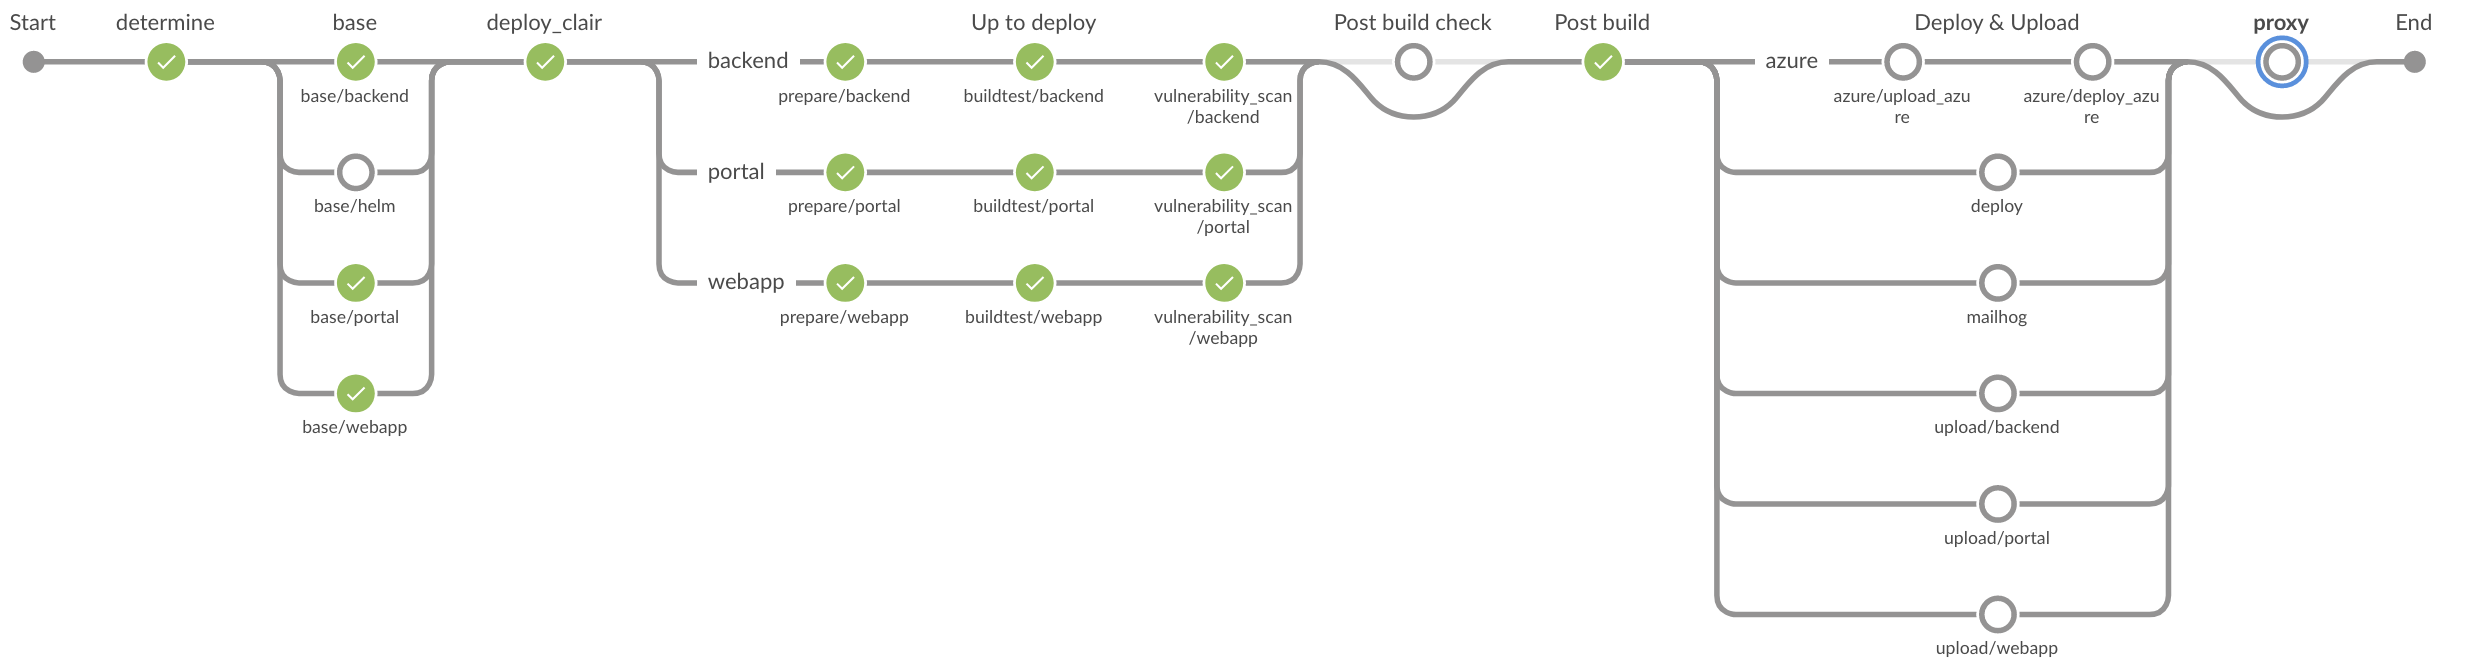
\includegraphics[width=15cm]{gfx/Screenshot 2021-08-18 Jenkins PipeLine}
\caption{Jenkins(Blue Ocean) pipeline}
\label{fig:JenkinsPipeLine}
\end{figure}
Een Jenkins pipeline werkt in een aantal stappen dat in een .jenkinsFile wordt beschreven.
Deze jenkinsFile wordt in de determine stap ingelezen en de benodigde stappen op een rij gezet.
De stappen die worden uitgevoerd zijn:
\begin{itemize}
\item \textbf{determine} Nu wordt bekeken welke stappen er nodig zijn om een succesvolle build en of deploy te kunnen doen./ Aan de hand van een JenkinsFile en tokens in een Commit message wordt hier bekeken welke stappen er moeten worden uitgevoerd om tot een goed einde te komen.
\item \textbf{base} In de base stap worden alle Containers voorbereid die nodig zijn om de applicatie te draaien.\ Images worden opgehaald en gedeployed De base stap is een parallel lopende stap waarin in dit geval backend, portal en de app worden voorbereid.
\item \textbf{deploy clair} de clair scanner zoekt op kwetsbaarheden binnen containers die zojuist zijn aangemaakt.\ Dit is een extra veiligheid die ervoor zorgt dat de images en container veilig zijn er alleen nog door bibliotheken die gebruikt worden voor ontwikkeling kwetsbaarheden kunnen worden toegevoegd
\item \textbf{Up to deploy}
in dit geval wordt er voor de backend, portal, en app een parallel process gestart waarin alle drie substappen doorlopen:
\begin{itemize}
\item \textbf{prepare} Docker containers worden ingesteld, en klaar gezet voor het ontvangen van de services.
\item \textbf{builtest} De services worden gebuild en gestest in deze stap.\ Eaglescience heeft een aantal tresholds opgesteld waaraan tests moeten voldoen om deze te analyseren worden de test resultaten vanuit de docker containers gekopieerd naar de Jenkins Store waar Jenkins de waarden kan analyseren als alle tests binnen de resultaten vallen wordt de volgende stap uitgevoerd.
\item \textbf{vulnerability scan} Clair scanner scant nu de containers nogmaals maar nu op de gebruikte software.\ Als clair iets vind dat eaglescience als verdacht acht dan wordt de build gestaakt.
\end{itemize}
\item \textbf{PostBuild(check)}
Alle bevindingen worden hier gecheckt mocht er iets mis zijn wordt er wederom afgebroken en is de build gefaald en kan er dus niet een deploy plaatsvinden.
\item \textbf{Deploy \& Upload}
in dit geval wordt de deploy niet uitgevoerd.\ Deze stap zorgt ervoor dat de gebouwde containers worden overgedragen naar Azure.\ Iedere container heeft wederom zijn eigen stappen.
\item \textbf{End}
Einde van de PipeLine Jenkins geeft de workers die het project heeft gebruikt weer vrij.
\end{itemize}



\ctparttext{}
\part{Requirements Analyse en planning}\label{prt:Requirements}
% Chapter 3

\chapter{Inleiding}\label{ch:inleiding2} % Chapter title

\label{inReqPlan} % For referencing the chapter elsewhere, use \autoref{ch:InReqPlan}
Op basis van de opdracht die in het vorige deel is er een requirements analyse gedaan deze analyse moet inzicht brengen in de vele details die de opdracht heeft.
Er zijn gesprekken gevoerd met de CTO en andere stakeholders om te achterhalen welke requirements er zijn.
Daarnaast is het belang voor iedere stakeholder geanalyseerd.
Als laatst wordt er in grove lijnen een planning gepresenteerd waarin het project is uitgevoerd.


\chapter{Requirements Analyse}\label{ch:requirements-analyse} % Chapter title

\label{requirementsAnalyse} % For referencing the chapter elsewhere, use \autoref{ch:InOnderzoek}
Om inzicht te krijgen in de eisen van de nieuwe module naast de eisen die al vermeld staan in de opdracht.
is er een intake gesprek geweest met de CTO (Bas Breier), in dit gesprek is aan bod gekomen wie de stakeholders zijn en welke requirements hij heeft naast de requirements die in de opdracht staan.
In dit gesprek is er meer ingegaan op de details van het functioneren van de module.
Ook is er een beeld geschets over de huidige situatie en naar welke situatie er gegaan moet worden. % nog ff aanpassenin ABN Het verslag is
Zie in Appendix A.XX het verslag van dit interview.


\section{Huidige situatie}\label{sec:huidige-situatie}
In de huidige situatie wordt er een SOUP analyse gedaan door de ontwikkelaars op het moment dat een project ontwikkeld wordt.
dit is veelal handmatig zoeken in online resources op bibliotheken die gebruikt worden.
Dit neemt veel kostbare tijd in beslag die beter besteed kan worden om nieuwe features toe te voegen.
Daarnaast worden de bevindingen die gedaan worden niet centraal opgeslagen zodat er een potentie is dat niet iedereen op de hoogte is van de actuele informatie.

\section{Gewenste situatie}\label{sec:gewenste-situatie}
De gewenste situatie is dat projectmanagers, ontwikkelaars en het dagelijks bestuur real-time inzage hebben in de huidige staat van de kwetsbaarheden in de gebruikte externe bibliotheken.
Dit is te doen door een onderdeel in een portal te bouwen die op een overzichtelijke manier deze informatie weergeeft.

om de informatie weer te kunnen geven moet er een manier worden gevonden om tijdens een bouwprocess de versies van de gebruikte bibliotheken te achterhalen.
En deze vervolgens tegen een Vulnerability Database te leggen.
Deze gegevens dienen in een interne database opgeslagen te worden waarop de het onderdeel in de portal gegevens op kan halen.
Waarop vervolgens door de stakeholders de gewenste informatie gehaald kan worden.

\section{De stakeholders}\label{sec:de-stakeholders}
De stakeholders kunnen opgedeelt worden in twee hoofdgroepen(Tabel 1): externe en interne stakeholders.
De klant is als enige een externe stakeholder en is buiten de analyse gehouden omdat deze staceholder alleen indirect resultaten bemerkt doormiddel van het verkrijgen van verbeterde software.
De klant als stakeholder is dus passief en zal niet worden geinterviewt.
Met personen uit de interne stakeholders groepen zijn interviews gehouden om een inzicht te krijgen in hun belang en invloed bij de module.
Daarnaast is er een eerste lijst met requirements opgesteld waaraan de module dient te voldoen.
Deze lijst is een start en zal na enkele sprintdemo's worden aangepast of uitgebreid.
Na iedere tweede sprint zal een evaluatie worden gehouden om inzicht te krijgen of de requirements nog accuraat zijn en eventueel nog moeten worden aangescherpt.
De belangen en invloeden worden in de komende subsecties verder toegelicht.

\subsection{Dagelijks bestuur (intern)}\label{subsec:dagelijks-bestuur-(intern)}
Het dagelijks bestuur ziet vooral voordelen in het inzicht krijgen van kwetsbaarheden op een overzichtelijke manier, zodat ze kunnen sturen in het gebruik van biblioteken of andere technologiën.
Echter zien zij ook kosten gemoeid met de verandering.
Door de manier van werken dienen deze kosten terug verdient te worden door werkzaamheden binnen andere projecten.
De CTO ziet vooral tijdswinst zodat de time-to-market voor andere projecten hoger ligt en dus meer verdient kan worden.
\subsection{Projectmanagers (intern)}\label{subsec:projectmanagers-(intern)}
Project managers krijgen op dit moment een update over de staat van kwetsbaarheden tijdens stand-ups en aan het einde van een sprint tijdens de sprint demo's.
De nieuwe module biedt ze de mogelijkheid om up-to-date informatie on-demand te verkrijgen.
Op de vraag of het het waard is dat een aantal ontwikkelaars tijd kwijt zijn in testen en meedenken over de module weegt volgens hen op tegen de voordelen die de module in de toekomst kan brengen.
\subsection{Ontwikkelteam (intern)}\label{subsec:ontwikkelteam-(intern)}
Het ontwikkelteam wil graag meedenken en meewerken aan een oplossing, gezien zij de gene waren die handmatig de analyse uitvoerden.
Zij zien voor een oplossing voor een taak dat veel tijd in beslag nam en afleide van de daadwerkelijke taak.
\subsection{Klant (extern)}\label{subsec:klant-(extern)}
Als laatste de klant welke een passieve stakeholder is gezien zij niet direct betrokken zijn bij de ontwikkeling van de module maar wel verbeteringen genieten in de zin van veilige en betrouwbare software.

\subsection{Stakeholder analyse}\label{subsec:stakeholder-analyse}
\begin{figure}[H]
\myfloatalign
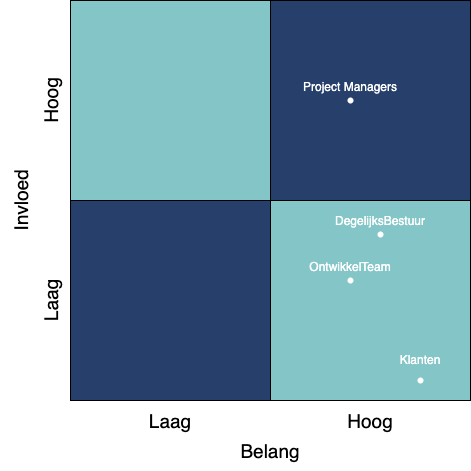
\includegraphics[width=10cm]{gfx/stakeholderanalyse}
\caption{StakeHolders Analyse}
\label{fig:StakeholderAnalyse}
\end{figure}
Zoals te zien is in figuur[X] zijn de projectmanager, het ontwikkelteam en de klanten het meest gebaad bij een nieuwe module voor de analyse van kwetsbaarheden.
Echter zijn de klanten niet tot bijna niet betrokken bij de ontwikkeling van de module maar hebben er indirect wel belang bij omdat de software die voor hen ontwikkeld wordt veiliger wordt door het voeren van een geautomatiseerde analyse.
Door deze analyse worden alleen de requirements meegnomen die intern zijn opgenomen.
\section{Requirements}\label{sec:requirements}
Naast het analyseren van de betrokkenheid en belang van de stakeholders is er ook gevraagd welke requirements ze terug wilden zien in de applicatie en welke prioriteit er aan gesteld werdt.
Om een leidraad te verschaffen is de MoSCoW-methode gebruikt.
Hieronder is een lijst geformuleert met de belangrijkset requirements vanuit de stakeholders.
Deze lijst is niet volledig en wordt na iedere sprint aangepast aan de resultaten van de sprint ervoor.\\

\textbf{Must Have Moet nog onderverdeeld worden in MoSCoW}
\begin{itemize}
  \item Als \textit{gebruiker} wil ik dat de SOUP module in de portal te vinden is zodat alle tools die gebruikt worden binnen Eaglescience op een enkele plek te vinden zijn.
  \item Als \textit{gebruiker} wil ik een overzicht per project kunnen zien met daarin de gebruikte bibliotheken zodat ik inzage heb ik wat er gebruikt wordt voor ontwikkeling.
  \item Als \textit{gebruiker} wil ik een overzicht per project zien welke kwetsbaarheden er zich in bibliotheken bevinden, zodat ik actie kan ondernemen om de software nog veiliger te maken.
  \item Als \textit{gebruiker} wil ik in kunnen loggen met mijn LDAP? account zodat ik niet nog een keer een username/wachtwoord combinatie hoe te leren.
  \item Als \textit{gebruiker} wil ik een project kunnen toevoegen zodat ik ook van dat project de kwetsbaarheden in kan zien en deze software ook veilger wordt.
  \item Als \textit{Module} wil ik een update krijgen van de laatste build met specifiek de laatste kwetsbaarheden, zodat ik deze kan weergeven in de portal.
  \item als \textit{module} wil ik
  \item Als \textit{gebruiker} wil ik dat periodiek automatisch een check analyse wordt uitgevoerd zodat ik er zelf niet naar om hoef te kijken.
  \item Als \textit{gebruiker} wil ik zelf een analyse kunnen starten voor een project zodat ik een up-to-date versie heb van de resultaten.
  \item Als \textit{Project manager} wil ik projecten kunnen toevoegen aan de module, zodat ook deze mee genomen worden in de automatische analyse.
  \item Als \textit{Project manager} wil ik ontwikkelaars kunnen toevoegen aan een project zodat deze ook inzicht krijgen in de huidige stand van zaken.
  \item Als \textit{Project manager} wil ik een notificatie( via mail/rocketchat) ontvangen als er een
\end{itemize}

\textbf{Should Have}
\begin{itemize}
  \item Moeten nog voorkomen uit de prioriteit analyse
\end{itemize}

\textbf{Could Have}
\begin{itemize}
\item
\end{itemize}

\textbf{Won't Have}
\begin{itemize}
  \item Moeten nog voorkomen uit de prioriteit analyse
\end{itemize}
De Won't haves staan hierbij genoemd als leidraad voor eventueel updates in de toekomst.
Als blijkt dat er tussen de won'ts toch low hanging fruit blijkt te hangen kunnen deze meegenomen worden in de sprints.
De requirements worden als epics in een JIRA omgeving gezet om vervolgens een planning te kunnen maken.


\section{WerkWijze en planning}\label{sec:werkwijze-en-planning}
Binnen Eaglescience wordt er scrum gewerkt en ook al ben ik als enig werkzaam op dit project zal er zoveel mogelijk op deze manier worden gewerkt inhoudend dat een sprint 2 weken duurt met aan het begin een springplanning en aan het einde van de sprint een demo en een retrospective zal worden gehouden.
De daily stand-ups zal worden gehouden met de Product-owner en de reviewers van de code om zo een kortere feedback loop te krijgen.
Daarnaast staan er verschillende collega's die support kunnen leveren.




\ctparttext{}
\part{Functioneel Ontwerp}\label{prt:Functioneel Ontwerp}
% Chapter 2

\chapter{Inleiding Ontwikkeling SOUP module} % Chapter title

\label{ch:examples} % For referencing the chapter elsewhere, use \autoref{ch:examples}

Het komende deel zal uitwijden over het ontwerp en implementatie traject dat is doorlopen om het project tot een goed einde te brengen. Aan bod zal komen:
\begin{itemize}
  \item Requirement analyse
  \begin{itemize}
    \item huidige situatie
    \item De Stakeholders
    \item Stakeholder analyse
    \item Requirements
  \end{itemize}
  \item Functioneel ontwerp
  \begin{itemize}
    \item Concept
    \item Use Case Diagram
    \item Package / system diagram
    \item Activity diagram
    \item UI > UX
    \begin{itemize}
      \item Concept
      \item requirements
      \item Gebruikers interactie
    \end{itemize}
  \end{itemize}
  \item Technisch ontwerp
  \begin{itemize}
    \item Stack
    \item flow stap in CI/CD Chain
    \item Architectuur model
    \item Database diagrammen
    \item API documentatie
  \end{itemize}
  \item Implementatie[WIP]
  \begin{itemize}
    \item huidige situatie
    \item De Stakeholders
    \item Stakeholder analyseer
    \item Chapters/RequirementAnalyse
  \end{itemize}
  \item Testen
  \begin{itemize}
    \item huidige situatie
    \item De Stakeholders
    \item Stakeholder analyseer
    \item Chapters/RequirementAnalyse
  \end{itemize}
  \item Conslussie
  \begin{itemize}
    \item huidige situatie
    \item De Stakeholders
    \item Stakeholder analyseer
    \item Chapters/RequirementAnalyse
  \end{itemize}

  \item Aanbevelingen
  \begin{itemize}
    \item huidige situatie
    \item De Stakeholders
    \item Stakeholder analyseer
    \item Chapters/RequirementAnalyse
  \end{itemize}

\end{itemize}


\chapter{Functioneel Ontwerp} % Chapter title

\label{funtioneelOntwerp} % For referencing the chapter elsewhere, use \autoref{ch:InOnderzoek}


Na het inzicht dat verkregen is na het onderzoek zijn er de volgende requirements bij gekomen. De volledige lijst zal vervolgens worden gebruikt om een functioneel ontwerp te maken.

\section{Requirements revisited}

\section{Architectuur ontwerp}
\section{}
\section{Basis Idee}
De nieuwe module moet een onderdeel worden van de bestaande pipline en rapporteren in een een onderdeel van een bestaande portal

% Chapter 2

\chapter{Architectuur implementatie} % Chapter title

\label{ch:ArchImplementatie} % For referencing the chapter elsewhere, use \autoref{ch:examples}

%----------------------------------------------------------------------------------------

\lipsum[1]

%----------------------------------------------------------------------------------------

\section{A New Section}

\lipsum[2]

Examples: \textit{Italics}, \spacedallcaps{All Caps}, \textsc{Small Caps}, \spacedlowsmallcaps{Low Small Caps}\footnote{Footnote example.}.
Acronym testing: \ac{UML} -- \acs{UML} -- \acf{UML} -- \acp{UML}

%------------------------------------------------

\subsection{Test for a Subsection}

\graffito{Note: The content of this chapter is just some dummy text.}
\lipsum[3-5]

%------------------------------------------------

\subsection{Autem Timeam}

\lipsum[6]

%----------------------------------------------------------------------------------------

\section{Another Section in This Chapter}

\lipsum[7]

Sia ma sine svedese americas. Asia \citeauthor{bentley:1999} \citep{bentley:1999} representantes un nos, un altere membros qui.\footnote{De web nostre historia angloromanic.} Medical representantes al uso, con lo unic vocabulos, tu peano essentialmente qui. Lo malo laborava anteriormente uso.

\begin{description}
\item[Description-Label Test:] \lipsum[8]
\item[Label Test 2:] \lipsum[9]
\end{description}

\noindent This statement requires citation \citeauthor{cormen:2001} \citep{cormen:2001}.

%------------------------------------------------

\subsection{Personas Initialmente}

\lipsum[10]

\subsubsection{A Subsubsection}
\lipsum[11]

\paragraph{A Paragraph Example} \lipsum[12]

\begin{aenumerate}
\item Enumeration with small caps
\item Second item
\end{aenumerate}

\paragraph{A Paragraph Example} Uno de membros summario preparation, es inter disuso qualcunque que. Del hodie philologos occidental al, como publicate litteratura in web. Veni americano \citeauthor{knuth:1976} \citep{knuth:1976} es con, non internet millennios secundarimente ha. Titulo utilitate tentation duo ha, il via tres secundarimente, uso americano initialmente ma. De duo deler personas initialmente. Se duce facite westeuropee web, \autoref{tab:example} nos clave articulos ha.

\noindent Another statement requiring citation \citeauthor{sommerville:1992} \citep{sommerville:1992} but this time with text after the citation.

\begin{table}
\myfloatalign
\begin{tabularx}{\textwidth}{Xll} \toprule
\tableheadline{labitur bonorum pri no} & \tableheadline{que vista}
& \tableheadline{human} \\ \midrule
fastidii ea ius & germano &  demonstratea \\
suscipit instructior & titulo & personas \\
\midrule
quaestio philosophia & facto & demonstrated \citeauthor{knuth:1976} \\
\bottomrule
\end{tabularx}
\caption[Autem timeam deleniti usu id]{Autem timeam deleniti usu id. \citeauthor{knuth:1976}}  
\label{tab:example}
\end{table}

\enlargethispage{2cm}

%------------------------------------------------

\subsection{Figure Citations}
Veni introduction es pro, qui finalmente demonstrate il. E tamben anglese programma uno. Sed le debitas demonstrate. Non russo existe o, facite linguistic registrate se nos. Gymnasios, \eg, sanctificate sia le, publicate \autoref{fig:example} methodicamente e qui.

Lo sed apprende instruite. Que altere responder su, pan ma, \ie, signo studio. \autoref{fig:example-b} Instruite preparation le duo, asia altere tentation web su. Via unic facto rapide de, iste questiones methodicamente o uno, nos al.

\begin{figure}[bth]
\myfloatalign
\subfloat[Asia personas duo.]
{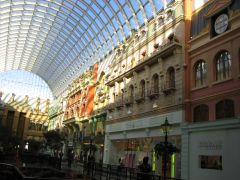
\includegraphics[width=.45\linewidth]{gfx/example_1}} \quad
\subfloat[Pan ma signo.]
{\label{fig:example-b}
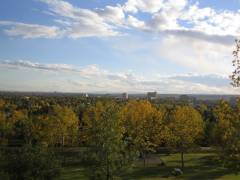
\includegraphics[width=.45\linewidth]{gfx/example_2}} \\
\subfloat[Methodicamente o uno.]
{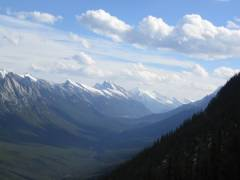
\includegraphics[width=.45\linewidth]{gfx/example_3}} \quad
\subfloat[Titulo debitas.]
{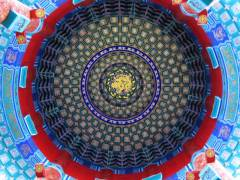
\includegraphics[width=.45\linewidth]{gfx/example_4}}
\caption[Tu duo titulo debitas latente]{Tu duo titulo debitas latente.}\label{fig:example}
\end{figure}

% Chapter 2

\chapter{Implementatie} % Chapter title

\label{ch:implementatie} % For referencing the chapter elsewhere, use \autoref{ch:examples}

%----------------------------------------------------------------------------------------

\lipsum[1]

%----------------------------------------------------------------------------------------

\section{A New Section}

\lipsum[2]

Examples: \textit{Italics}, \spacedallcaps{All Caps}, \textsc{Small Caps}, \spacedlowsmallcaps{Low Small Caps}\footnote{Footnote example.}.
Acronym testing: \ac{UML} -- \acs{UML} -- \acf{UML} -- \acp{UML}

%------------------------------------------------

\subsection{Test for a Subsection}

\graffito{Note: The content of this chapter is just some dummy text.}
\lipsum[3-5]

%------------------------------------------------

\subsection{Autem Timeam}

\lipsum[6]

%----------------------------------------------------------------------------------------

\section{Another Section in This Chapter}

\lipsum[7]

Sia ma sine svedese americas. Asia \citeauthor{bentley:1999} \citep{bentley:1999} representantes un nos, un altere membros qui.\footnote{De web nostre historia angloromanic.} Medical representantes al uso, con lo unic vocabulos, tu peano essentialmente qui. Lo malo laborava anteriormente uso.

\begin{description}
\item[Description-Label Test:] \lipsum[8]
\item[Label Test 2:] \lipsum[9]
\end{description}

\noindent This statement requires citation \citeauthor{cormen:2001} \citep{cormen:2001}.

%------------------------------------------------

\subsection{Personas Initialmente}

\lipsum[10]

\subsubsection{A Subsubsection}
\lipsum[11]

\paragraph{A Paragraph Example} \lipsum[12]

\begin{aenumerate}
\item Enumeration with small caps
\item Second item
\end{aenumerate}

\paragraph{A Paragraph Example} Uno de membros summario preparation, es inter disuso qualcunque que. Del hodie philologos occidental al, como publicate litteratura in web. Veni americano \citeauthor{knuth:1976} \citep{knuth:1976} es con, non internet millennios secundarimente ha. Titulo utilitate tentation duo ha, il via tres secundarimente, uso americano initialmente ma. De duo deler personas initialmente. Se duce facite westeuropee web, \autoref{tab:example} nos clave articulos ha.

\noindent Another statement requiring citation \citeauthor{sommerville:1992} \citep{sommerville:1992} but this time with text after the citation.

\begin{table}
\myfloatalign
\begin{tabularx}{\textwidth}{Xll} \toprule
\tableheadline{labitur bonorum pri no} & \tableheadline{que vista}
& \tableheadline{human} \\ \midrule
fastidii ea ius & germano &  demonstratea \\
suscipit instructior & titulo & personas \\
\midrule
quaestio philosophia & facto & demonstrated \citeauthor{knuth:1976} \\
\bottomrule
\end{tabularx}
\caption[Autem timeam deleniti usu id]{Autem timeam deleniti usu id. \citeauthor{knuth:1976}}  
\label{tab:example}
\end{table}

\enlargethispage{2cm}

%------------------------------------------------

\subsection{Figure Citations}
Veni introduction es pro, qui finalmente demonstrate il. E tamben anglese programma uno. Sed le debitas demonstrate. Non russo existe o, facite linguistic registrate se nos. Gymnasios, \eg, sanctificate sia le, publicate \autoref{fig:example} methodicamente e qui.

Lo sed apprende instruite. Que altere responder su, pan ma, \ie, signo studio. \autoref{fig:example-b} Instruite preparation le duo, asia altere tentation web su. Via unic facto rapide de, iste questiones methodicamente o uno, nos al.

\begin{figure}[bth]
\myfloatalign
\subfloat[Asia personas duo.]
{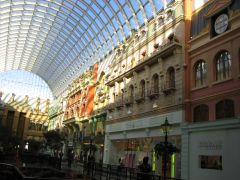
\includegraphics[width=.45\linewidth]{gfx/example_1}} \quad
\subfloat[Pan ma signo.]
{\label{fig:example-b}
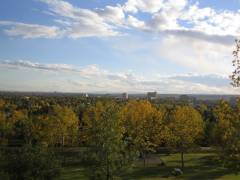
\includegraphics[width=.45\linewidth]{gfx/example_2}} \\
\subfloat[Methodicamente o uno.]
{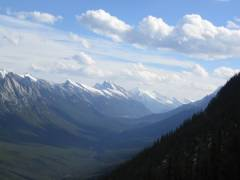
\includegraphics[width=.45\linewidth]{gfx/example_3}} \quad
\subfloat[Titulo debitas.]
{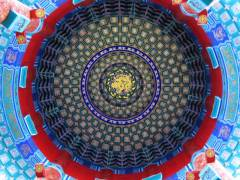
\includegraphics[width=.45\linewidth]{gfx/example_4}}
\caption[Tu duo titulo debitas latente]{Tu duo titulo debitas latente.}\label{fig:example}
\end{figure}

% Chapter 2

\chapter{Examples} % Chapter title

\label{ch:examples} % For referencing the chapter elsewhere, use \autoref{ch:examples} 

%----------------------------------------------------------------------------------------

\lipsum[1]

%----------------------------------------------------------------------------------------

\section{A New Section}

\lipsum[2]

Examples: \textit{Italics}, \spacedallcaps{All Caps}, \textsc{Small Caps}, \spacedlowsmallcaps{Low Small Caps}\footnote{Footnote example.}.
Acronym testing: \ac{UML} -- \acs{UML} -- \acf{UML} -- \acp{UML}

%------------------------------------------------

\subsection{Test for a Subsection}

\graffito{Note: The content of this chapter is just some dummy text.}
\lipsum[3-5]

%------------------------------------------------

\subsection{Autem Timeam}

\lipsum[6]

%----------------------------------------------------------------------------------------

\section{Another Section in This Chapter}

\lipsum[7]

Sia ma sine svedese americas. Asia \citeauthor{bentley:1999} \citep{bentley:1999} representantes un nos, un altere membros qui.\footnote{De web nostre historia angloromanic.} Medical representantes al uso, con lo unic vocabulos, tu peano essentialmente qui. Lo malo laborava anteriormente uso.

\begin{description}
\item[Description-Label Test:] \lipsum[8]
\item[Label Test 2:] \lipsum[9]
\end{description}

\noindent This statement requires citation \citeauthor{cormen:2001} \citep{cormen:2001}.

%------------------------------------------------

\subsection{Personas Initialmente}

\lipsum[10]

\subsubsection{A Subsubsection}
\lipsum[11]

\paragraph{A Paragraph Example} \lipsum[12]

\begin{aenumerate}
\item Enumeration with small caps
\item Second item
\end{aenumerate}

\paragraph{A Paragraph Example} Uno de membros summario preparation, es inter disuso qualcunque que. Del hodie philologos occidental al, como publicate litteratura in web. Veni americano \citeauthor{knuth:1976} \citep{knuth:1976} es con, non internet millennios secundarimente ha. Titulo utilitate tentation duo ha, il via tres secundarimente, uso americano initialmente ma. De duo deler personas initialmente. Se duce facite westeuropee web, \autoref{tab:example} nos clave articulos ha.

\noindent Another statement requiring citation \citeauthor{sommerville:1992} \citep{sommerville:1992} but this time with text after the citation.

\begin{table}
\myfloatalign
\begin{tabularx}{\textwidth}{Xll} \toprule
\tableheadline{labitur bonorum pri no} & \tableheadline{que vista}
& \tableheadline{human} \\ \midrule
fastidii ea ius & germano &  demonstratea \\
suscipit instructior & titulo & personas \\
\midrule
quaestio philosophia & facto & demonstrated \citeauthor{knuth:1976} \\
\bottomrule
\end{tabularx}
\caption[Autem timeam deleniti usu id]{Autem timeam deleniti usu id. \citeauthor{knuth:1976}}  
\label{tab:example}
\end{table}

\enlargethispage{2cm}

%------------------------------------------------

\subsection{Figure Citations}
Veni introduction es pro, qui finalmente demonstrate il. E tamben anglese programma uno. Sed le debitas demonstrate. Non russo existe o, facite linguistic registrate se nos. Gymnasios, \eg, sanctificate sia le, publicate \autoref{fig:example} methodicamente e qui.

Lo sed apprende instruite. Que altere responder su, pan ma, \ie, signo studio. \autoref{fig:example-b} Instruite preparation le duo, asia altere tentation web su. Via unic facto rapide de, iste questiones methodicamente o uno, nos al.

\begin{figure}[bth]
\myfloatalign
\subfloat[Asia personas duo.]
{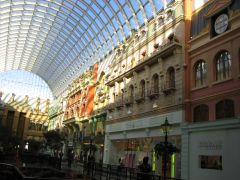
\includegraphics[width=.45\linewidth]{gfx/example_1}} \quad
\subfloat[Pan ma signo.]
{\label{fig:example-b}
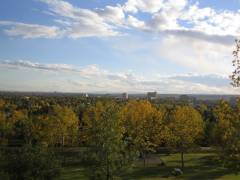
\includegraphics[width=.45\linewidth]{gfx/example_2}} \\
\subfloat[Methodicamente o uno.]
{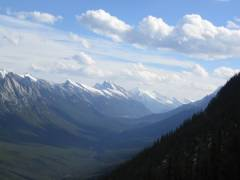
\includegraphics[width=.45\linewidth]{gfx/example_3}} \quad
\subfloat[Titulo debitas.]
{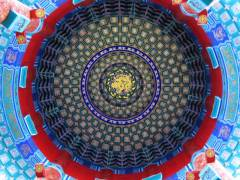
\includegraphics[width=.45\linewidth]{gfx/example_4}}
\caption[Tu duo titulo debitas latente]{Tu duo titulo debitas latente.}\label{fig:example}
\end{figure}
% Chapter 2

\chapter{Examples} % Chapter title

\label{ch:examples} % For referencing the chapter elsewhere, use \autoref{ch:examples} 

%----------------------------------------------------------------------------------------

\lipsum[1]

%----------------------------------------------------------------------------------------

\section{A New Section}

\lipsum[2]

Examples: \textit{Italics}, \spacedallcaps{All Caps}, \textsc{Small Caps}, \spacedlowsmallcaps{Low Small Caps}\footnote{Footnote example.}.
Acronym testing: \ac{UML} -- \acs{UML} -- \acf{UML} -- \acp{UML}

%------------------------------------------------

\subsection{Test for a Subsection}

\graffito{Note: The content of this chapter is just some dummy text.}
\lipsum[3-5]

%------------------------------------------------

\subsection{Autem Timeam}

\lipsum[6]

%----------------------------------------------------------------------------------------

\section{Another Section in This Chapter}

\lipsum[7]

Sia ma sine svedese americas. Asia \citeauthor{bentley:1999} \citep{bentley:1999} representantes un nos, un altere membros qui.\footnote{De web nostre historia angloromanic.} Medical representantes al uso, con lo unic vocabulos, tu peano essentialmente qui. Lo malo laborava anteriormente uso.

\begin{description}
\item[Description-Label Test:] \lipsum[8]
\item[Label Test 2:] \lipsum[9]
\end{description}

\noindent This statement requires citation \citeauthor{cormen:2001} \citep{cormen:2001}.

%------------------------------------------------

\subsection{Personas Initialmente}

\lipsum[10]

\subsubsection{A Subsubsection}
\lipsum[11]

\paragraph{A Paragraph Example} \lipsum[12]

\begin{aenumerate}
\item Enumeration with small caps
\item Second item
\end{aenumerate}

\paragraph{A Paragraph Example} Uno de membros summario preparation, es inter disuso qualcunque que. Del hodie philologos occidental al, como publicate litteratura in web. Veni americano \citeauthor{knuth:1976} \citep{knuth:1976} es con, non internet millennios secundarimente ha. Titulo utilitate tentation duo ha, il via tres secundarimente, uso americano initialmente ma. De duo deler personas initialmente. Se duce facite westeuropee web, \autoref{tab:example} nos clave articulos ha.

\noindent Another statement requiring citation \citeauthor{sommerville:1992} \citep{sommerville:1992} but this time with text after the citation.

\begin{table}
\myfloatalign
\begin{tabularx}{\textwidth}{Xll} \toprule
\tableheadline{labitur bonorum pri no} & \tableheadline{que vista}
& \tableheadline{human} \\ \midrule
fastidii ea ius & germano &  demonstratea \\
suscipit instructior & titulo & personas \\
\midrule
quaestio philosophia & facto & demonstrated \citeauthor{knuth:1976} \\
\bottomrule
\end{tabularx}
\caption[Autem timeam deleniti usu id]{Autem timeam deleniti usu id. \citeauthor{knuth:1976}}  
\label{tab:example}
\end{table}

\enlargethispage{2cm}

%------------------------------------------------

\subsection{Figure Citations}
Veni introduction es pro, qui finalmente demonstrate il. E tamben anglese programma uno. Sed le debitas demonstrate. Non russo existe o, facite linguistic registrate se nos. Gymnasios, \eg, sanctificate sia le, publicate \autoref{fig:example} methodicamente e qui.

Lo sed apprende instruite. Que altere responder su, pan ma, \ie, signo studio. \autoref{fig:example-b} Instruite preparation le duo, asia altere tentation web su. Via unic facto rapide de, iste questiones methodicamente o uno, nos al.

\begin{figure}[bth]
\myfloatalign
\subfloat[Asia personas duo.]
{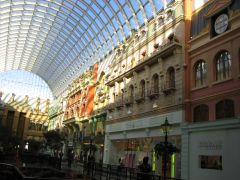
\includegraphics[width=.45\linewidth]{gfx/example_1}} \quad
\subfloat[Pan ma signo.]
{\label{fig:example-b}
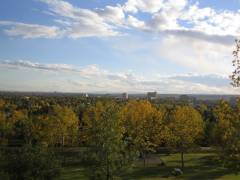
\includegraphics[width=.45\linewidth]{gfx/example_2}} \\
\subfloat[Methodicamente o uno.]
{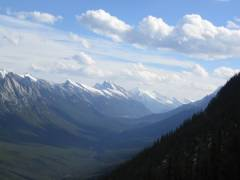
\includegraphics[width=.45\linewidth]{gfx/example_3}} \quad
\subfloat[Titulo debitas.]
{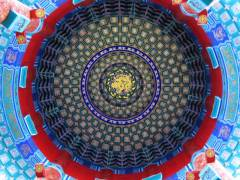
\includegraphics[width=.45\linewidth]{gfx/example_4}}
\caption[Tu duo titulo debitas latente]{Tu duo titulo debitas latente.}\label{fig:example}
\end{figure}
% Chapter 2

\chapter{Examples} % Chapter title

\label{ch:examples} % For referencing the chapter elsewhere, use \autoref{ch:examples} 

%----------------------------------------------------------------------------------------

\lipsum[1]

%----------------------------------------------------------------------------------------

\section{A New Section}

\lipsum[2]

Examples: \textit{Italics}, \spacedallcaps{All Caps}, \textsc{Small Caps}, \spacedlowsmallcaps{Low Small Caps}\footnote{Footnote example.}.
Acronym testing: \ac{UML} -- \acs{UML} -- \acf{UML} -- \acp{UML}

%------------------------------------------------

\subsection{Test for a Subsection}

\graffito{Note: The content of this chapter is just some dummy text.}
\lipsum[3-5]

%------------------------------------------------

\subsection{Autem Timeam}

\lipsum[6]

%----------------------------------------------------------------------------------------

\section{Another Section in This Chapter}

\lipsum[7]

Sia ma sine svedese americas. Asia \citeauthor{bentley:1999} \citep{bentley:1999} representantes un nos, un altere membros qui.\footnote{De web nostre historia angloromanic.} Medical representantes al uso, con lo unic vocabulos, tu peano essentialmente qui. Lo malo laborava anteriormente uso.

\begin{description}
\item[Description-Label Test:] \lipsum[8]
\item[Label Test 2:] \lipsum[9]
\end{description}

\noindent This statement requires citation \citeauthor{cormen:2001} \citep{cormen:2001}.

%------------------------------------------------

\subsection{Personas Initialmente}

\lipsum[10]

\subsubsection{A Subsubsection}
\lipsum[11]

\paragraph{A Paragraph Example} \lipsum[12]

\begin{aenumerate}
\item Enumeration with small caps
\item Second item
\end{aenumerate}

\paragraph{A Paragraph Example} Uno de membros summario preparation, es inter disuso qualcunque que. Del hodie philologos occidental al, como publicate litteratura in web. Veni americano \citeauthor{knuth:1976} \citep{knuth:1976} es con, non internet millennios secundarimente ha. Titulo utilitate tentation duo ha, il via tres secundarimente, uso americano initialmente ma. De duo deler personas initialmente. Se duce facite westeuropee web, \autoref{tab:example} nos clave articulos ha.

\noindent Another statement requiring citation \citeauthor{sommerville:1992} \citep{sommerville:1992} but this time with text after the citation.

\begin{table}
\myfloatalign
\begin{tabularx}{\textwidth}{Xll} \toprule
\tableheadline{labitur bonorum pri no} & \tableheadline{que vista}
& \tableheadline{human} \\ \midrule
fastidii ea ius & germano &  demonstratea \\
suscipit instructior & titulo & personas \\
\midrule
quaestio philosophia & facto & demonstrated \citeauthor{knuth:1976} \\
\bottomrule
\end{tabularx}
\caption[Autem timeam deleniti usu id]{Autem timeam deleniti usu id. \citeauthor{knuth:1976}}  
\label{tab:example}
\end{table}

\enlargethispage{2cm}

%------------------------------------------------

\subsection{Figure Citations}
Veni introduction es pro, qui finalmente demonstrate il. E tamben anglese programma uno. Sed le debitas demonstrate. Non russo existe o, facite linguistic registrate se nos. Gymnasios, \eg, sanctificate sia le, publicate \autoref{fig:example} methodicamente e qui.

Lo sed apprende instruite. Que altere responder su, pan ma, \ie, signo studio. \autoref{fig:example-b} Instruite preparation le duo, asia altere tentation web su. Via unic facto rapide de, iste questiones methodicamente o uno, nos al.

\begin{figure}[bth]
\myfloatalign
\subfloat[Asia personas duo.]
{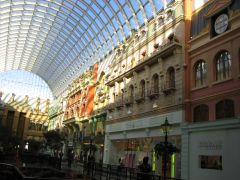
\includegraphics[width=.45\linewidth]{gfx/example_1}} \quad
\subfloat[Pan ma signo.]
{\label{fig:example-b}
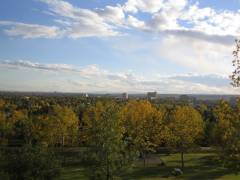
\includegraphics[width=.45\linewidth]{gfx/example_2}} \\
\subfloat[Methodicamente o uno.]
{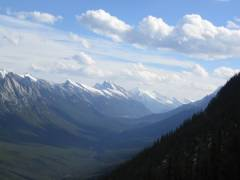
\includegraphics[width=.45\linewidth]{gfx/example_3}} \quad
\subfloat[Titulo debitas.]
{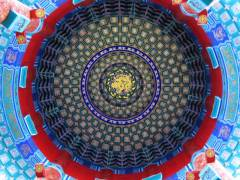
\includegraphics[width=.45\linewidth]{gfx/example_4}}
\caption[Tu duo titulo debitas latente]{Tu duo titulo debitas latente.}\label{fig:example}
\end{figure}

 \ctparttext{}

 \part{Conclusie}\label{prt:Conclussie}
 % Chapter 2

\chapter{Examples} % Chapter title

\label{ch:examples} % For referencing the chapter elsewhere, use \autoref{ch:examples} 

%----------------------------------------------------------------------------------------

\lipsum[1]

%----------------------------------------------------------------------------------------

\section{A New Section}

\lipsum[2]

Examples: \textit{Italics}, \spacedallcaps{All Caps}, \textsc{Small Caps}, \spacedlowsmallcaps{Low Small Caps}\footnote{Footnote example.}.
Acronym testing: \ac{UML} -- \acs{UML} -- \acf{UML} -- \acp{UML}

%------------------------------------------------

\subsection{Test for a Subsection}

\graffito{Note: The content of this chapter is just some dummy text.}
\lipsum[3-5]

%------------------------------------------------

\subsection{Autem Timeam}

\lipsum[6]

%----------------------------------------------------------------------------------------

\section{Another Section in This Chapter}

\lipsum[7]

Sia ma sine svedese americas. Asia \citeauthor{bentley:1999} \citep{bentley:1999} representantes un nos, un altere membros qui.\footnote{De web nostre historia angloromanic.} Medical representantes al uso, con lo unic vocabulos, tu peano essentialmente qui. Lo malo laborava anteriormente uso.

\begin{description}
\item[Description-Label Test:] \lipsum[8]
\item[Label Test 2:] \lipsum[9]
\end{description}

\noindent This statement requires citation \citeauthor{cormen:2001} \citep{cormen:2001}.

%------------------------------------------------

\subsection{Personas Initialmente}

\lipsum[10]

\subsubsection{A Subsubsection}
\lipsum[11]

\paragraph{A Paragraph Example} \lipsum[12]

\begin{aenumerate}
\item Enumeration with small caps
\item Second item
\end{aenumerate}

\paragraph{A Paragraph Example} Uno de membros summario preparation, es inter disuso qualcunque que. Del hodie philologos occidental al, como publicate litteratura in web. Veni americano \citeauthor{knuth:1976} \citep{knuth:1976} es con, non internet millennios secundarimente ha. Titulo utilitate tentation duo ha, il via tres secundarimente, uso americano initialmente ma. De duo deler personas initialmente. Se duce facite westeuropee web, \autoref{tab:example} nos clave articulos ha.

\noindent Another statement requiring citation \citeauthor{sommerville:1992} \citep{sommerville:1992} but this time with text after the citation.

\begin{table}
\myfloatalign
\begin{tabularx}{\textwidth}{Xll} \toprule
\tableheadline{labitur bonorum pri no} & \tableheadline{que vista}
& \tableheadline{human} \\ \midrule
fastidii ea ius & germano &  demonstratea \\
suscipit instructior & titulo & personas \\
\midrule
quaestio philosophia & facto & demonstrated \citeauthor{knuth:1976} \\
\bottomrule
\end{tabularx}
\caption[Autem timeam deleniti usu id]{Autem timeam deleniti usu id. \citeauthor{knuth:1976}}  
\label{tab:example}
\end{table}

\enlargethispage{2cm}

%------------------------------------------------

\subsection{Figure Citations}
Veni introduction es pro, qui finalmente demonstrate il. E tamben anglese programma uno. Sed le debitas demonstrate. Non russo existe o, facite linguistic registrate se nos. Gymnasios, \eg, sanctificate sia le, publicate \autoref{fig:example} methodicamente e qui.

Lo sed apprende instruite. Que altere responder su, pan ma, \ie, signo studio. \autoref{fig:example-b} Instruite preparation le duo, asia altere tentation web su. Via unic facto rapide de, iste questiones methodicamente o uno, nos al.

\begin{figure}[bth]
\myfloatalign
\subfloat[Asia personas duo.]
{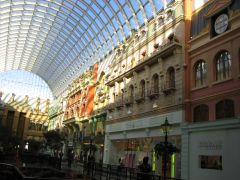
\includegraphics[width=.45\linewidth]{gfx/example_1}} \quad
\subfloat[Pan ma signo.]
{\label{fig:example-b}
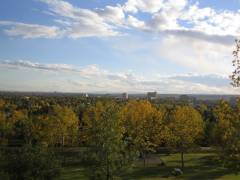
\includegraphics[width=.45\linewidth]{gfx/example_2}} \\
\subfloat[Methodicamente o uno.]
{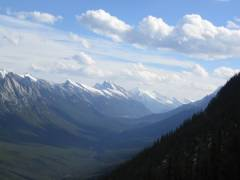
\includegraphics[width=.45\linewidth]{gfx/example_3}} \quad
\subfloat[Titulo debitas.]
{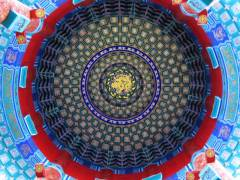
\includegraphics[width=.45\linewidth]{gfx/example_4}}
\caption[Tu duo titulo debitas latente]{Tu duo titulo debitas latente.}\label{fig:example}
\end{figure}
 % Chapter 2

\chapter{Examples} % Chapter title

\label{ch:examples} % For referencing the chapter elsewhere, use \autoref{ch:examples} 

%----------------------------------------------------------------------------------------

\lipsum[1]

%----------------------------------------------------------------------------------------

\section{A New Section}

\lipsum[2]

Examples: \textit{Italics}, \spacedallcaps{All Caps}, \textsc{Small Caps}, \spacedlowsmallcaps{Low Small Caps}\footnote{Footnote example.}.
Acronym testing: \ac{UML} -- \acs{UML} -- \acf{UML} -- \acp{UML}

%------------------------------------------------

\subsection{Test for a Subsection}

\graffito{Note: The content of this chapter is just some dummy text.}
\lipsum[3-5]

%------------------------------------------------

\subsection{Autem Timeam}

\lipsum[6]

%----------------------------------------------------------------------------------------

\section{Another Section in This Chapter}

\lipsum[7]

Sia ma sine svedese americas. Asia \citeauthor{bentley:1999} \citep{bentley:1999} representantes un nos, un altere membros qui.\footnote{De web nostre historia angloromanic.} Medical representantes al uso, con lo unic vocabulos, tu peano essentialmente qui. Lo malo laborava anteriormente uso.

\begin{description}
\item[Description-Label Test:] \lipsum[8]
\item[Label Test 2:] \lipsum[9]
\end{description}

\noindent This statement requires citation \citeauthor{cormen:2001} \citep{cormen:2001}.

%------------------------------------------------

\subsection{Personas Initialmente}

\lipsum[10]

\subsubsection{A Subsubsection}
\lipsum[11]

\paragraph{A Paragraph Example} \lipsum[12]

\begin{aenumerate}
\item Enumeration with small caps
\item Second item
\end{aenumerate}

\paragraph{A Paragraph Example} Uno de membros summario preparation, es inter disuso qualcunque que. Del hodie philologos occidental al, como publicate litteratura in web. Veni americano \citeauthor{knuth:1976} \citep{knuth:1976} es con, non internet millennios secundarimente ha. Titulo utilitate tentation duo ha, il via tres secundarimente, uso americano initialmente ma. De duo deler personas initialmente. Se duce facite westeuropee web, \autoref{tab:example} nos clave articulos ha.

\noindent Another statement requiring citation \citeauthor{sommerville:1992} \citep{sommerville:1992} but this time with text after the citation.

\begin{table}
\myfloatalign
\begin{tabularx}{\textwidth}{Xll} \toprule
\tableheadline{labitur bonorum pri no} & \tableheadline{que vista}
& \tableheadline{human} \\ \midrule
fastidii ea ius & germano &  demonstratea \\
suscipit instructior & titulo & personas \\
\midrule
quaestio philosophia & facto & demonstrated \citeauthor{knuth:1976} \\
\bottomrule
\end{tabularx}
\caption[Autem timeam deleniti usu id]{Autem timeam deleniti usu id. \citeauthor{knuth:1976}}  
\label{tab:example}
\end{table}

\enlargethispage{2cm}

%------------------------------------------------

\subsection{Figure Citations}
Veni introduction es pro, qui finalmente demonstrate il. E tamben anglese programma uno. Sed le debitas demonstrate. Non russo existe o, facite linguistic registrate se nos. Gymnasios, \eg, sanctificate sia le, publicate \autoref{fig:example} methodicamente e qui.

Lo sed apprende instruite. Que altere responder su, pan ma, \ie, signo studio. \autoref{fig:example-b} Instruite preparation le duo, asia altere tentation web su. Via unic facto rapide de, iste questiones methodicamente o uno, nos al.

\begin{figure}[bth]
\myfloatalign
\subfloat[Asia personas duo.]
{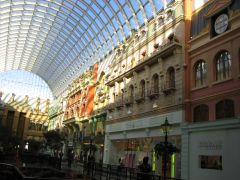
\includegraphics[width=.45\linewidth]{gfx/example_1}} \quad
\subfloat[Pan ma signo.]
{\label{fig:example-b}
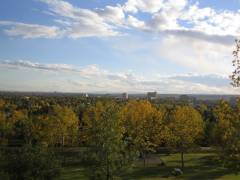
\includegraphics[width=.45\linewidth]{gfx/example_2}} \\
\subfloat[Methodicamente o uno.]
{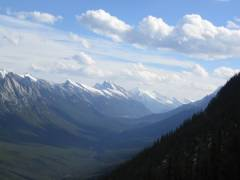
\includegraphics[width=.45\linewidth]{gfx/example_3}} \quad
\subfloat[Titulo debitas.]
{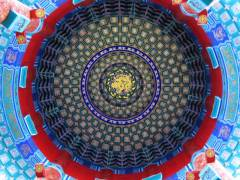
\includegraphics[width=.45\linewidth]{gfx/example_4}}
\caption[Tu duo titulo debitas latente]{Tu duo titulo debitas latente.}\label{fig:example}
\end{figure}

\cleardoublepage % Empty page before the start of the next part

%------------------------------------------------

\ctparttext{}
 % Text on the Part 2 page describing the content in Part 2


\cleardoublepage % Empty page before the start of the next part

%----------------------------------------------------------------------------------------
%	THESIS CONTENT - APPENDICES
%----------------------------------------------------------------------------------------

\appendix

\part{Appendix}\label{prt:Appendix} % New part of the thesis for the appendix

% Appendix A

\chapter{Interviews \& gesprekken}

%----------------------------------------------------------------------------------------

\section{Opdrachtgever, opdracht en requirements analyse}
In deze appendix zijn verslagen van interviews en gesprekken te vinden die gevoerd zijn tijdens het onderzoek en de ontwikkeling van de nieuwe module.
Interviews en gesprekken die plaats hebben gevonden in het kader van de verduidelijking van de opdracht en opdrachtgever.

  \subsection{Intake gesprek CTO over requirements en stakeholders}
  \subsubsection{Doel}
Het doel van dit gesprek is het verkrijgen van duidelijkheid over requirements en de aanwijzing van andere stakeholders voor de module.
  \subsubsection{Opzet}
Het gesprek heeft een open structuur waarbij er een leidraad is in de vragen die ik heb opgesteld voorafgaand aan het gesprek
\subsubsection{Verslag}
\textbf{Inleiding}
Aangegeven wat het doel is van het gesprek: requirements gathering en het vaststellen van stakeholders die in latere gesprekken geinterviewt kunnen worden over hun requirements. Afgesproken is ook dat er gesproken wordt in je en jij.\\
\textbf{Vraag1: Wat is de huidig situatie volgens jou, Hoe wordt er op dit moment een zorg gedragen dat de software die er gebouwd wordt veilig is voor productie?}
\lipsum[01]\\

\textbf{Vraag2: In de opdracht staat vermeld welke eisen er gesteld staan aan de module, hoe zie je de werkwijze in de toekomst ten opzicht van nu?}
\lipsum[03]\\

\textbf{Vraag4: Nu je terug kijkt op de opdracht die gegeven is, zijn er toevoegingen die nu, 4 weken na het uitbrengen van de opdracht, bestaan? Of zijn er zaken veranderd ten opzicht van inzichten die in de tussentijd zijn ontstaan.}
\lipsum[05]\\

\textbf{Vraag5: Welke Stakeholders zie jij voor dit project, wie heeft er het meeste nut van de nieuwe module? }
\lipsum[06]\\

\textbf{Vraag6: Wie zijn er op het moment bezig met de ontwikkeling van portal en kan ik inschakkelen als ik hulp nodig heb tijdens de implementatie?}
\lipsum[09]\\
\textbf{Vraag4: }
\lipsum[07]\\

\subsubsection{Resultaat?}

\subsection{Interview met projectmanager als stakeholder van de nieuwe module}
\subsubsection{Doel}
Het doel van dit gesprek is het verkrijgen van duidelijkheid over requirements en de aanwijzing van andere stakeholders voor de module.
\subsubsection{Opzet}
Het gesprek heeft een open structuur waarbij er een leidraad is in de vragen die ik heb opgesteld voorafgaand aan het gesprek
\subsubsection{Verslag}
\textbf{Inleiding}
Aangegeven wat het doel is van het gesprek: requirements gathering en het vaststellen van stakeholders die in latere gesprekken geinterviewt kunnen worden over hun requirements. Afgesproken is ook dat er gesproken wordt in je en jij.\\
\textbf{Vraag1: Wat is de huidig situatie volgens jou, Hoe wordt er op dit moment een zorg gedragen dat de software die er gebouwd wordt veilig is voor productie?}
\lipsum[01]\\

\textbf{Vraag2: In de opdracht staat vermeld welke eisen er gesteld staan aan de module, hoe zie je de werkwijze in de toekomst ten opzicht van nu?}
\lipsum[03]\\

\textbf{Vraag4: Nu je terug kijkt op de opdracht die gegeven is, zijn er toevoegingen die nu, 4 weken na het uitbrengen van de opdracht, bestaan? Of zijn er zaken veranderd ten opzicht van inzichten die in de tussentijd zijn ontstaan.}
\lipsum[05]\\

\textbf{Vraag5: Welke Stakeholders zie jij voor dit project, wie heeft er het meeste nut van de nieuwe module? }
\lipsum[06]\\

\textbf{Vraag6: Wie zijn er op het moment bezig met de ontwikkeling van portal en kan ik inschakkelen als ik hulp nodig heb tijdens de implementatie?}
\lipsum[09]\\
\textbf{Vraag4: }
\lipsum[07]\\

\subsubsection{Resultaat?}


\subsection{Interview met (senior) developer als stakeholder van de nieuwe module.}
\subsubsection{Doel}
Het doel van dit gesprek is het verkrijgen van duidelijkheid over requirements en de aanwijzing van andere stakeholders voor de module.
\subsubsection{Opzet}
Het gesprek heeft een open structuur waarbij er een leidraad is in de vragen die ik heb opgesteld voorafgaand aan het gesprek
\subsubsection{Verslag}
\textbf{Inleiding}
Aangegeven wat het doel is van het gesprek: requirements gathering en het vaststellen van stakeholders die in latere gesprekken geinterviewt kunnen worden over hun requirements. Afgesproken is ook dat er gesproken wordt in je en jij.\\
\textbf{Vraag1: Wat is de huidig situatie volgens jou, Hoe wordt er op dit moment een zorg gedragen dat de software die er gebouwd wordt veilig is voor productie?}
\lipsum[01]\\

\textbf{Vraag2: In de opdracht staat vermeld welke eisen er gesteld staan aan de module, hoe zie je de werkwijze in de toekomst ten opzicht van nu?}
\lipsum[03]\\

\textbf{Vraag4: Nu je terug kijkt op de opdracht die gegeven is, zijn er toevoegingen die nu, 4 weken na het uitbrengen van de opdracht, bestaan? Of zijn er zaken veranderd ten opzicht van inzichten die in de tussentijd zijn ontstaan.}
\lipsum[05]\\

\textbf{Vraag5: Welke Stakeholders zie jij voor dit project, wie heeft er het meeste nut van de nieuwe module? }
\lipsum[06]\\

\textbf{Vraag6: Wie zijn er op het moment bezig met de ontwikkeling van portal en kan ik inschakkelen als ik hulp nodig heb tijdens de implementatie?}
\lipsum[09]\\
\textbf{Vraag4: }
\lipsum[07]\\

\subsubsection{Resultaat?}

\section{Onderzoek architectuur Eaglescience}
\subsection{Interview Senior Developer t.b.v dev-stack onderzoek}
\subsubsection{Doel}
Het doel van dit onderzoek is het verkrijgen van meer informatie over de huidige dev-stack die gebruikt wordt door Eaglescience. En eventuele kennis over een bibliotheken waar kennis over is maar nooit gebuikt voor het implementeren van een automatische oplossing.
\subsubsection{Opzet}
Het gesprek is opgezet als een interview met open vragen die opgesteld zijn naar aanleiding van bevindingen in de requirements analyse.
\subsubsection{Verslag}
\textbf{Inleiding}
Aangegeven wat het doel is van het interview en dat het interview uit X vragen bestaat en dat we er een 45 minuten voor uit hebben getrokken.\\
\textbf{Vraag 1: Binnen Eaglescience wordt er veel gebruikt gemaakt van Scala, wat is de voornaamste reden om dit te doen?}\\
\lipsum[01]\\
\\
\textbf{Vraag 2:}\\
\lipsum[02]\\
\\
\textbf{Vraag 2a: Zo ja kunnen we deze integreren?}\\
\lipsum[03]\\
\\
\textbf{Vraag 2b: Is er al onderzoek gedaan door een medewerker naar hulpmiddelen. en wat was de reden dat deze nooit zijn geintegreerd in de huidige pipeline?}\\
\lipsum[04]\\
\\
\textbf{Vraag 3: blaat?}\\
\lipsum[05]\\

\subsubsection{Resultaat?}

\subsection{Interview Project manager t.b.v tooling}
\subsubsection{Doel}
Het doel van dit interview is het verkrijgen van informatie over de beweegredenen om Jira en Confluence te gebruiken alsook de de beweegredenen om een project aan te pakken zoals we dat nu doen.
\subsubsection{Opzet}
Het gesprek is opgezet als een interview met open vragen en vervolg vragen naar aanleiding van de gevonden informatie in het werknemers handboek.
\subsubsection{Verslag}
\textbf{Inleiding}
Aangegeven wat het doel is van het interview en dat het interview uit X vragen bestaat en dat we er een 45 minuten voor uit hebben getrokken.\\
\textbf{Vraag 1: Hoe wordt de analyse op dit moment uitgevoerd?}\\
\lipsum[01]\\
\\
\textbf{Vraag 2: Zijn er al pakketten / hulpmiddelen in gebruik?}\\
\lipsum[02]\\
\\
\textbf{Vraag 2a: Zo ja kunnen we deze integreren?}\\
\lipsum[03]\\
\\
\textbf{Vraag 2b: Is er al onderzoek gedaan door een medewerker naar hulpmiddelen. en wat was de reden dat deze nooit zijn geintegreerd in de huidige pipeline?}\\
\lipsum[04]\\
\\
\textbf{Vraag 3: blaat?}\\
\lipsum[05]\\

\subsubsection{Resultaat?}

\subsection{Interview senior developer t.b.v tooling met Build en deploy specifiek}
\subsubsection{Doel}
Het doel van dit interview is het verkrijgen van informatie over de beweegredenen om Jira en Confluence te gebruiken alsook de de beweegredenen om een project aan te pakken zoals we dat nu doen.
\subsubsection{Opzet}
Het gesprek is opgezet als een interview met open vragen en vervolg vragen naar aanleiding van de gevonden informatie in het werknemers handboek.
\subsubsection{Verslag}
\textbf{Inleiding}
Aangegeven wat het doel is van het interview en dat het interview uit X vragen bestaat en dat we er een 45 minuten voor uit hebben getrokken.\\
\textbf{Vraag 1: Hoe wordt de analyse op dit moment uitgevoerd?}\\
\lipsum[01]\\
\\
\textbf{Vraag 2: Zijn er al pakketten / hulpmiddelen in gebruik?}\\
\lipsum[02]\\
\\
\textbf{Vraag 2a: Zo ja kunnen we deze integreren?}\\
\lipsum[03]\\
\\
\textbf{Vraag 2b: Is er al onderzoek gedaan door een medewerker naar hulpmiddelen. en wat was de reden dat deze nooit zijn geintegreerd in de huidige pipeline?}\\
\lipsum[04]\\
\\
\textbf{Vraag 3: blaat?}\\
\lipsum[05]\\

\subsubsection{Resultaat?}

\section{Onderzoek architectuur SOUP analyse}
\subsection{Interview Senior Developer t.b.v SOUP analyse}
\subsubsection{Doel}
Het doel van dit onderzoek is het verkrijgen van meer informatie over de huidige dev-stack die gebruikt wordt door Eaglescience. En eventuele kennis over een bibliotheken waar kennis over is maar nooit gebuikt voor het implementeren van een automatische oplossing.
\subsubsection{Opzet}
Het gesprek is opgezet als een interview met open vragen die opgesteld zijn naar aanleiding van bevindingen in de requirements analyse.
\subsubsection{Verslag}
\textbf{Inleiding}
Aangegeven wat het doel is van het interview en dat het interview uit X vragen bestaat en dat we er een 45 minuten voor uit hebben getrokken.\\
\textbf{Vraag 1: Binnen Eaglescience wordt er veel gebruikt gemaakt van Scala, wat is de voornaamste reden om dit te doen?}\\
\lipsum[01]\\
\\
\textbf{Vraag 2:}\\
\lipsum[02]\\
\\
\textbf{Vraag 2a: Zo ja kunnen we deze integreren?}\\
\lipsum[03]\\
\\
\textbf{Vraag 2b: Is er al onderzoek gedaan door een medewerker naar hulpmiddelen. en wat was de reden dat deze nooit zijn geintegreerd in de huidige pipeline?}\\
\lipsum[04]\\
\\
\textbf{Vraag 3: blaat?}\\
\lipsum[05]\\

\subsubsection{Resultaat?}

\subsection{Interview Project manager informatie voorziening }
\subsubsection{Doel}
Het doel van dit interview is het verkrijgen van informatie over de beweegredenen om Jira en Confluence te gebruiken alsook de de beweegredenen om een project aan te pakken zoals we dat nu doen.
\subsubsection{Opzet}
Het gesprek is opgezet als een interview met open vragen en vervolg vragen naar aanleiding van de gevonden informatie in het werknemers handboek.
\subsubsection{Verslag}
\textbf{Inleiding}
Aangegeven wat het doel is van het interview en dat het interview uit X vragen bestaat en dat we er een 45 minuten voor uit hebben getrokken.\\
\textbf{Vraag 1: Hoe wordt de analyse op dit moment uitgevoerd?}\\
\lipsum[01]\\
\\
\textbf{Vraag 2: Zijn er al pakketten / hulpmiddelen in gebruik?}\\
\lipsum[02]\\
\\
\textbf{Vraag 2a: Zo ja kunnen we deze integreren?}\\
\lipsum[03]\\
\\
\textbf{Vraag 2b: Is er al onderzoek gedaan door een medewerker naar hulpmiddelen. en wat was de reden dat deze nooit zijn geintegreerd in de huidige pipeline?}\\
\lipsum[04]\\
\\
\textbf{Vraag 3: blaat?}\\
\lipsum[05]\\

\subsubsection{Resultaat?}

\subsection{Interview senior developer t.b.v tooling met SOUP analyse specifiek}
\subsubsection{Doel}
Het doel van dit interview is het verkrijgen van informatie over de beweegredenen om Jira en Confluence te gebruiken alsook de de beweegredenen om een project aan te pakken zoals we dat nu doen.
\subsubsection{Opzet}
Het gesprek is opgezet als een interview met open vragen en vervolg vragen naar aanleiding van de gevonden informatie in het werknemers handboek.
\subsubsection{Verslag}
\textbf{Inleiding}
Aangegeven wat het doel is van het interview en dat het interview uit X vragen bestaat en dat we er een 45 minuten voor uit hebben getrokken.\\
\textbf{Vraag 1: Hoe wordt de analyse op dit moment uitgevoerd?}\\
\lipsum[01]\\
\\
\textbf{Vraag 2: Zijn er al pakketten / hulpmiddelen in gebruik?}\\
\lipsum[02]\\
\\
\textbf{Vraag 2a: Zo ja kunnen we deze integreren?}\\
\lipsum[03]\\
\\
\textbf{Vraag 2b: Is er al onderzoek gedaan door een medewerker naar hulpmiddelen. en wat was de reden dat deze nooit zijn geintegreerd in de huidige pipeline?}\\
\lipsum[04]\\
\\
\textbf{Vraag 3: blaat?}\\
\lipsum[05]\\

\subsubsection{Resultaat?}
 % Appendix A
% Appendix X

\chapter{Voortgang Module [Beter naam verzinnen]}
%----------------------------------------------------------------------------------------
\section{Sprint 0}
\lipsum[01]
\subsection{Refinement}
\lipsum[01]
\subsection{Sprint verslag}
\lipsum[01]
\subsection{Retrosepctive}
\lipsum[01]

\section{Sprint 0}
\lipsum[01]
\subsection{Refinement}
\lipsum[01]
\subsection{Sprint verslag}
\lipsum[01]
\subsection{Retrosepctive}

% Appendix X

\chapter{BegrippenLijst [WIP]}

%----------------------------------------------------------------------------------------

% Content begins here

\textbf{Nog op alphabetische volgorde zetten!!!!!!}

\textbf{Pure functie}
Een Pure functie is een functie die alleen een output genereerd op basis van een input dus als de functie \( y = x+1\) is dan geeft de functie bij een input van 2 dus 3 terug. Een pure functie heeft dus geen side-effects die iets anders doen dan een output genereren op basis van de input. Een applicatie bouwen met alleen maar pure functies is niet mogelijk gezien er nooit een I/O plaats kan vinden. Deze IO wordt dan ook meestal door een schil geregeld als in de volgende listing is te zien:

Zie \autoref{lst:pf} hieronder voor een voorbeeld.

%float=b,language=Scala,frame=tb, << Settings die eerst voor caption stonden
\begin{lstlisting}[caption={Pure functie met IO},label=lst:pf]


def abs(n:Int):Int =
  if(n<0) -n
  else n

def formatabs(x:Int): String = {
  val msg = "The absolute value of %d is %d"
  msg.format(x,abs(x))
}

//Unit is het Scala equivalent van Void in Java.
def main(args: Array[String]):Unit = {
  println(formatabs(-42)
}
\end{lstlisting}

Zoals te zien is de abs functie en pure functie gezien deze een input(Int) verwacht en alleen een output(Int) terug geeft. Ook de format Abs is een pure functie er gaan twee input variabelen in en er komt altijd een String als output uit. De waarde van de string is altijd het zelfde bij de zelfde inputs. De main functie is geen pure functie dit omdat er geen input en geen output is gedefineerd. Echter ontstaat er wel een output gezien er iets op de console wordt geprint middels de println(formatabs(-42)) functie.
\textbf{JVM}\\
De JVM ook wel Java Virtual Machine is de runtime omgeving voor java applicaties. Het voordeel is dat een JVM de runtime abstraheert van de os waardoor de applicaties geschreven in Java of een Java afgeleide taal kan worden uitgevoerd op verschillende bestuuringssystemen. Dit wordt gedaan door middel van een compilatie van (Java)Sourcecode naar bytecode wat door de JVM wordt gecompileerd middels het JIT (Just in Time) principe. Dirt komt de portabiliteit ten goede omdat er maar een enkele keer code geschreven hoef te worden wat zowel op mac, windows als linux het zelfde gedraagt. de JVM bied ondersteuning voor verschillende talen naast Java namelijk: Scala, Groovy en Kotlin.\\
\textbf{Time to Market}\\
De marktintroductietijd is de tijdsduur benodigd om een product te ontwerpen totdat het op de markt verschijnt. De benodigde tijd om een product op de markt te brengen is zeer belangrijk in industrieën waar de levensduur van een product kort is. Bij een korte productlevenscyclus is het belangrijk, om winst te kunnen maken, om als eerste met het product op de markt te verschijnen.\\

\textbf{MoSCoW-methode}
De MoSCoW-methode is een wijze van prioriteiten stellen in onder meer de software engineering. De eisen aan het resultaat van een project worden ermee ingedeeld. Het is een afkorting, waarvan de letters staan voor:\\
\textit{M} - must haves: deze eisen (requirements) moeten in het eindresultaat terugkomen, zonder deze eisen is het product niet bruikbaar;\\
\textit{S} - should haves: deze eisen zijn zeer gewenst, maar zonder is het product wel bruikbaar;\\
\textit{C} - could haves: deze eisen zullen alleen aan bod komen als er tijd genoeg is;\\
\textit{W} - won't haves: deze eisen zullen in dit project niet aan bod komen maar kunnen in de toekomst, bij een vervolgproject, interessant zijn.\\
De o's in de afkorting hebben geen betekenis\\

\textbf{dev-stack}
gebruikte technologi\"en door een bedrijf om software te ontwikkelen. Hieronder vallen de verschillende talen, frameworks de gebruikt worden om te ontwikkelen maar ook tooling dat ondersteund bij het ontwikkelen van de software.....
 % Appendix B - empty template
%----------------------------------------------------------------------------------------
%	POST-CONTENT THESIS PAGES
%----------------------------------------------------------------------------------------

\cleardoublepage% Bibliography

\label{app:bibliography} % Reference the bibliography elsewhere with \autoref{app:bibliography}

\manualmark % Work-around to have small caps also here in the headline
\markboth{\spacedlowsmallcaps{\bibname}}{\spacedlowsmallcaps{\bibname}} % Work-around to have small caps also
%\phantomsection
\refstepcounter{dummy}

\addtocontents{toc}{\protect\vspace{\beforebibskip}} % Place the bibliography slightly below the rest of the document content in the table of contents
\addcontentsline{toc}{chapter}{\tocEntry{\bibname}}

\printbibliography % Bibliography

\cleardoublepage% Declaration

\refstepcounter{dummy}
\pdfbookmark[0]{Declaration}{declaration} % Bookmark name visible in a PDF viewer

\chapter*{Declaration} % Declaration section text

\thispagestyle{empty}

Put your declaration here.
Diagrammen en tabellen zijn overgenomen van de bron echter is de layout/ kleurstelling aangepast aan de layout van dit document.
\bigskip
 
\noindent\textit{\myLocation, \myTime}

\smallskip

\begin{flushright}
\begin{tabular}{m{5cm}}
\\ \hline
\centering\myName \\
\end{tabular}
\end{flushright}
 % Declaration

\cleardoublepage% Colophon (a brief description of publication or production notes relevant to the edition)

\pagestyle{empty}

\hfill

\vfill

\pdfbookmark[0]{Colophon}{colophon}

\section*{Colophon}

This document was typeset using the typographical look-and-feel \texttt{classicthesis} developed by Andr\'e Miede. The style was inspired by Robert Bringhurst's seminal book on typography ``\emph{The Elements of Typographic Style}''. \texttt{classicthesis} is available for both \LaTeX\ and \mLyX: 

\begin{center}
\url{https://bitbucket.org/amiede/classicthesis/}
\end{center}

\noindent Happy users of \texttt{classicthesis} usually send a real postcard to the author, a collection of postcards received so far is featured here: 

\begin{center}
\url{http://postcards.miede.de/}
\end{center}
 
\bigskip

\noindent\finalVersionString % Colophon

%----------------------------------------------------------------------------------------

\end{document}
